\documentclass[11pt, ngerman]{article}
\usepackage{cite}
\usepackage{url}
\usepackage{amsmath}
\usepackage{amsfonts}
\usepackage{cleveref}
\usepackage{xstring}
\usepackage{trfsigns}
\usepackage{verbatim}
\usepackage{listings}
\usepackage{graphicx}
\usepackage{xcolor}
\usepackage{caption}
\usepackage{float}


\crefname{equation}{Gleichung}{Gleichungen}

\lstset{breaklines=true,language=C, basicstyle=\footnotesize, keywordstyle=\color{blue}, basicstyle=\footnotesize, numbers=left, stepnumber=1, morekeywords={kernel, global, local, constant, const}}

\begin{document}

\newcommand*{\Ef}[3]{%
	\IfEqCase{#3}{%
		{+}{E_{#1}^{#2}\vert_{t+\Delta t}}%
		{-}{E_{#1}^{#2}\vert_{t-\Delta t}}%
		{0}{E_{#1}^{#2}\vert_{t}}%
		{T}{E_{#1}^{#2}\vert_{T}}%
	}[\PackageError{tree}{Undefined option to Ef: #1}{}]%
}

\newcommand*{\Hf}[3]{%
	\IfEqCase{#3}{%
		{+}{\widetilde{H_{#1}}^{#2}\vert_{t+\frac{\Delta t}{2}}}%
		{-}{\widetilde{H_{#1}}^{#2}\vert_{t-\frac{\Delta t}{2}}}%
		{0}{\widetilde{H_{#1}}^{#2}\vert_{t}}%
		{T}{\widetilde{H_{#1}}^{#2}\vert_{T}}%
	}[\PackageError{tree}{Undefined option to Hf: #1}{}]%
}

\newcommand*{\Ch}[3]{%
	\IfEqCase{#3}{%
		{+}{C_{#1}^H\vert_{t+\frac{\Delta t}{2}}^{#2}}%
		{-}{C_{#1}^H\vert_{t-\frac{\Delta t}{2}}^{#2}}%
		{0}{C_{#1}^H\vert_{t}^{#2}}%
		{T}{C_{#1}^H\vert_{T}^{#2}}%
		{T+}{C_{#1}^H\vert_{T+\frac{\Delta t}{2}}^{#2}}%
	}[\PackageError{tree}{Undefined option to Cf: #1}{}]%
}

\newcommand*{\Ce}[3]{%
	\IfEqCase{#3}{%
		{+}{C_{#1}^E\vert_{t+\frac{\Delta t}{2}}^{#2}}%
		{-}{C_{#1}^E\vert_{t-\frac{\Delta t}{2}}^{#2}}%
		{0}{C_{#1}^E\vert_{t}^{#2}}%
		{T}{C_{#1}^E\vert_{T}^{#2}}%
		{T+}{C_{#1}^E\vert_{T+\frac{\Delta t}{2}}^{#2}}%
	}[\PackageError{tree}{Undefined option to Cf: #1}{}]%
}

\newcommand*{\dt}[3]{%
	\begin{bmatrix}
		{#1} & 0 & 0\\
		0 & {#2} & 0\\
		0 & 0 & {#3}
	\end{bmatrix}
}

\newcommand*{\sgma}{\sigma^`}
\newcommand*{\sollsein}{\stackrel{!}{=}}

\newcommand*{\mone}{\frac{\sgma_y+\sgma_z}{2\epsilon_0} + \frac{\sgma_y\sgma_z\Delta t}{4\epsilon_0} + \frac{1}{\Delta t}}
\newcommand*{\fone}{-\frac{\sgma_y+\sgma_z}{2\epsilon_0} + \frac{\sgma_y\sgma_z\Delta t}{4\epsilon_0} + \frac{1}{\Delta t}}

\newcommand{\source}[1]{\caption*{Source: {#1}} }

\begin{titlepage}
	\begin{center}
		\begin{Large}Hardwarebeschleunigte elektromagnetische Simulation einer Drahtantenne\end{Large}
		\vfill
		\begin{Large}Bachelorarbeit -- HTW Berlin\end{Large}
		\vfill
		\begin{Small}Lukas Brumm (S0553370)\\1. und 2. Pr\"ufer: Udo Pursche, Heiko H\"ubert\\Datum: 11.03.19\end{Small}
	\end{center}
\end{titlepage}

\date{}
\maketitle
\tableofcontents
\newpage

\section{Einleitung}
Die vorliegende Arbeit `Hardwarebeschleunigte elektromagnetische Simulation von Drahtantennen'
wurde im Rahmen des Studienganges `Informations- und 
Kommunikationstechnik' an der Hochschule f\"ur Technik und Wirtschaft Berlin
verfasst. Ziel der Arbeit ist es die Methode der finiten Differenzen
im Zeitbereich (FDTD-Methode) nachzuvollziehen und f\"ur eine
hardwarebeschleunigte Simulation von Drahtantennen zu verwenden.
Ich hiehlt mich bei der Herleitung der FDTD-Methode an die Vorlesung
`Electromagnetic Analysis Using Finite-Difference Time-Domain'
samt ver\"offentlichtem Skript Raymond Rumpfs der Universit\"at
Texas in El Paso\cite{methode}, wobei ich mich entschloss die Maxwellgleichungen f\"ur
ein normalisiertes H-Feld zu l\"osen und nur auf dem E- und H-Feld zu arbeiten.
Dadurch l\"asst sich die numerische L\"osung der Maxwellgleichungen
durch nur zwei Formeln g\"anzlich beschreiben.

\section{Motivation}
Jede drahtlose Kommunikation ben\"otigt eine Antenne auf der
Sende und Empfangsseite. Durch die fortschreitende Miniaturisierung
der Elektronik und eine daraus folgende Vernetzung 
wie man sie zum Beispiel im Internet of Things (IoT)
beobachten kann, werden immer spezifischere Charakteristiken
an die Sende- und Empfangsantenne gestellt. In solchen Einsatzgebieten
sind konventionelle Antennendesigns h\"aufig nicht anwendbar,
sondern erfordern spezielle Antennen. Der Entwurf solcher Antennen
passiert interaktiv mit einem Simulationsprogramm, wobei auch
gezeigt wurde, dass evolution\"are Algorithmen (EA) zum automatisierten
Antennendesign verwendet werden k\"onnen.\cite{nasa_ea_antenna}
Ein solcher EA muss mitunter hunderttausende Simulationen durchf\"uhren\cite[p.6]{nasa_ea_antenna},
weshalb jede Simulation so performant wie m\"oglich sein sollte.

\section{Stand der Technik}
Das numerische L\"osen von Differentialgleichungnen wird seit 1928 untersucht
\cite{fdtd_u} und hat sich seitdem kontinuierlich weiterentwickelt.\cite{fdtd_history}
Neben der FDTD existieren noch andere Verfahren, um Differentialgleichungen
zu l\"osen, wie zum Beispiel die Finite-Elemente-Methode, die Finite-Volumen-Methode,
oder die Randelement-Methode, die h\"aufig f\"ur Differentialgleichungen
besonderer Form entwickelt wurde\cite{mathepedia_numerische_verfahren}.
Die FDTD-Methode hingegen kann auf beliebige Differentialgleichungen angewandt
werden und wird im Verlaufe der Arbeit eingehend behandelt.
Auch wenn die FDTD-Methode seit 1928 erforscht wird, werden f\"ur die Einsatzgebiete
der FDTD noch immer neue Erkenntisse gewonnen, so ist zum Beispiel die Simulation einer Antenneneinspeisung
noch nicht vollst\"andig gekl\"art und wird weiterhin untersucht\cite{advanced_gap_feed}.

\section{L\"osen der Maxwellgleichungen durch die FDTD-Methode}
Die FDTD-Methode, auch Yee-Methode genannt, l\"ost Differentialgleichungen
indem die als infinitesimal klein angenommenen Differentialquotienten
durch finite Differenzenquotienten approximiert werden.~\cite{fdtd_u}
Die Maxwellgleichungen werden daher nur in der Differentialform betrachtet.
Die FDTD-Methode ist zu komplex und problemabh\"angig,
als dass eine Einsch\"atzung der Simulationsergebnise gelingen k\"onnte, ohne die FDTD-Methode
mathematisch f\"ur ein Problem nachvollzogen zu haben.
Es werden daher nun kurz die Maxwellgleichungen eingef\"uhrt, allgemeine
Stabilit\"atsbedingungen der FDTD-Methode behandelt und die FDTD-Methode
genutzt, um eine numerische L\"osung der Maxwellgleichungen sowie des
`Perfectly Matched Layer' (PML) herzuleiten.

\subsection{Maxwellgleichungen}
Unter den Maxwellgleichungen versteht man die folgenden Gleichungen, die
zusammen alle elektromagnetischen Ph\"anomene beschreiben.
Das Gau{\ss}-Gesetz f\"ur Elektrizit\"at\cite{gausz_law_electric},

\begin{equation}
	\nabla * \vec{D} = \rho_v
	\label{eq:gausz_law_e}
\end{equation}
wobei \(\vec{D}\) die elektrische Flussdichte und \(\rho_v\) die Ladungsdichte ist.
Elektrische Felder divergieren bei positiven Ladungen und konvergieren bei negativen
Ladungen. Das Gau{\ss}-Gesetz f\"ur Magnetismus\cite{gausz_law_magnetic},

\begin{align}
	\nabla * \vec{B} = 0
	\label{eq:gausz_law_h}
\end{align}
wobei \(\vec{B}\) die magnetische Flussdichte ist.
Es gibt keine magnetischen Monopole, Magnetfelder formen immer Schleifen.
Das Amperesche Gesetz\cite{amperes_law},

\begin{align}
	\nabla\times\vec{H} = \vec{J} + \frac{\partial\vec{D}}{\partial t}
\end{align}
wobei \(\vec{H}\) das magnetische Feld und \(\vec{J}\) die Stromdichte ist.
Zirkulierende magnetishe Felder induzieren Str\"ome sowie zeitabh\"angige
elektrische Felder. Das Induktionsgesetz\cite{induction_law},

\begin{align}
	\nabla\times\vec{E} = -\frac{\partial\vec{B}}{\partial t}
\end{align}
wobei \(\vec{E}\) das elektrische Feld ist.
Zirkulierende elektrische Felder induzieren zeitabh\"angige magnetische Felder.
Weiterhin ist das D-Feld \"uber die Permittivit\"at mit dem E-Feld verbunden,\cite{constitutive}

\begin{align}
	\vec{D}(t) = [\epsilon(t)] * \vec{E}(t)
	\label{eq:constitutive1}
\end{align}
sowie das B-Feld \"uber die Permeabilit\"at mit dem H-Feld verbunden ist.\cite{constitutive}

\begin{align}
	\vec{B}(t) = [\mu(t)] * \vec{E}(t)
	\label{eq:constitutive2}
\end{align}
In beiden F\"allen handelt es sich um eine Faltung mit einem Tensor.
Im Verlauf der Arbeit wird angenommen, dass die Permittivit\"at und die Permeabilit\"at zeitlich
konstant sind, damit wird die Faltung zu einer Multiplikation. Verwendet man die
\cref{eq:constitutive1,eq:constitutive2} um das D- und B-Feld zu eliminieren und
gibt man die Permittivit\"at und Permeabilit\"at relativ zur Vacuumpermittivit\"at und
-permeabilit\"at an, so ergeben sich folgende vier Formeln.

\begin{align}
	&\nabla * ([\mu]\vec{H}(t)) = 0 \\
	&\nabla * ([\epsilon]\vec{E}(t)) = \rho_v \\
	&\nabla\times\vec{H} = \epsilon_0[\epsilon_r]\frac{\partial\vec{E}}{\partial t} \label{eq:nabla_h} \\
	&\nabla\times\vec{E} = -\mu_0[\mu_r]\frac{\partial\vec{H}}{\partial t} \label{eq:nabla_e}
\end{align}
Aus den beiden verschr\"ankten \cref{eq:nabla_h,eq:nabla_e} werden sp\"ater die sog.
Updategleichungen hergeleitet, also die Gleichungen die das E- bezw. H-Feld des n\"achsten
Zeitschrittes liefern. Die Stromdichte \(\vec{J}\) kann genutzt werden, um
Verlust innerhalb von Materialien darzustellen. Im Verlauf der Arbeit wird angenommen,
dass die Antennengeometrie nicht verlustbehaftet ist.

\begin{align}
	\vec{J} = 0
\end{align}
Das E- und H-Feld sind durch die Materialimpedanz \(\eta\) mit einander verkn\"upft, wobei jede
Impedanz relativ zur Freiraumimpedanz \(\eta_0\) angegeben werden kann:

\begin{align}
	\eta &= \frac{|\vec{E}|}{|\vec{H}|}\\
	\eta &= \eta_0 * \sqrt{\frac{\mu_r}{\epsilon_r}}, \eta_0 = \pi*119,9169832\Omega
\end{align}
Im freien Raum ist das E- Feld also um den Faktor \(\eta_0\) gr\"o{\ss}er als das H-Feld.
Diese Skalierung f\"uhrt bei numerischen L\"osungsverfahren zu Rundungsfehlern,
weshalb das H-Feld normalisiert wird und somit die gleiche Gr\"o{\ss}enordnung wie das
E-Feld besitzt.\cite{normalize_h_field}

\begin{align}
	\widetilde{\vec{H}} &= \eta_0\vec{H}\\
	\vec{H} &= \frac{1}{\eta_0}\widetilde{\vec{H}}
\end{align}
\newpage
\noindent Somit ergibt sich aus \cref{eq:nabla_e}:

\begin{align}
	\nabla\times\vec{E} &= [-\mu]\frac{\partial\widetilde{\vec{H}}}{\partial t} * \frac{1}{\eta_0}\quad\vert \eta_0 = \mu_0 * c\nonumber\\
	&=-\mu_0[\mu_r]\frac{1}{\mu_0c}\frac{\partial\widetilde{\vec{H}}}{\partial t}\nonumber\\
	&=-\frac{[\mu_r]}{c}\frac{\partial\widetilde{\vec{H}}}{\partial t}
\end{align}
Und aus \cref{eq:nabla_h} ergibt sich:

\begin{align}
	\nabla\times\widetilde{\vec{H}} &= \eta_0\epsilon_0[\epsilon_r]\frac{\partial\vec{E}}{\partial t}\nonumber\\
	&= c\mu_0\epsilon_0[\epsilon_r]\frac{\partial\vec{E}}{\partial t}\quad\vert \mu_0 = \frac{1}{c^2\epsilon_0}\nonumber\\
	&= \frac{1}{c^2\epsilon_0}c\epsilon_0[\epsilon_r]\frac{\partial\vec{E}}{\partial t}\nonumber\\
	&= \frac{[\epsilon_r]}{c}\frac{\partial\vec{E}}{\partial t}
\end{align}


\subsection{Mathematische Stabilit\"atsbedingungen f\"ur finite Differenzen}
Immer wenn die FDTD-Methode auf Differentialgleichungen angewendet
wird muss jede finite-Differenz am selben Punkt im Raum und in der
Zeit existieren, um die Differentialgleichung korrekt zu approximieren.\cite{fdtd_stabilitaet}

\begin{align}
	\frac{\partial f(x)}{\partial x} + f(x) &= 0 \vert FDTD-Methode \\
	\underbrace{\frac{x + \Delta x - f(x)}{\Delta x}}_{\mathrm{Existiert\ am\ Punkt\ x + \frac{\Delta x}{2}}} + \underbrace{f(x)}_{Existiert\ am\ Punkt\ x} &= 0\quad\vert x = n\Delta x, x \in \mathbb{N}  
\end{align}
Diese Gleichung w\"are instabil, der Term \(f(x)\) muss interpoliert werden um ebenfalls
an den Punkten \(x + \frac{\Delta x}{2}\) zu existieren:

\begin{align}
	\frac{f(x + \Delta x) - f(x)}{\Delta x} + \frac{f(x + \Delta x) + f(x)}{2} &= 0
\end{align}

\subsection{Anwenden der FDTD auf die Maxwellgleichungen}
Die \cref{eq:nabla_h,eq:nabla_e} beinhalten eine offensichtliche Ableitung nach
der Zeit und eine Ableitung nach allen drei Dimensionen, die im \(\nabla\)-Operator
steckt:

\begin{align}
	\nabla &= (\frac{\partial}{\partial x_1}, \ldots, \frac{\partial}{\partial x_n})
\end{align}
Als erstes wird die Ableitung nach der Zeit betrachted und mit der FDTD-Methode approximiert:

\begin{align}
	\nabla\times\vec{E}(t) &= -\frac{[\mu_r]}{c}\frac{\partial\widetilde{\vec{H}}(t)}{\partial t}\quad\vert FDTD-Methode \\
	\underbrace{\nabla\times\vec{E}(t)}_{\mathrm{Zeitpunkt\ t}} &= \underbrace{-\frac{[\mu_r]}{c}\frac{\widetilde{\vec{H}}(t+\Delta t)-\widetilde{\vec{H}}(t)}{\Delta t}}_{Zeitpunkt\ t+\frac{\Delta t}{2}} \\
	\nabla\times\widetilde{\vec{H}}(t) &= \frac{\epsilon_r}{c}\frac{\partial\vec{E}(t)}{\partial t}\quad\vert FDTD-Methode \\
	\underbrace{\nabla\times\widetilde{\vec{H}}(t)}_{\mathrm{Zeitpunkt\ t}} &= \underbrace{\frac{\epsilon_r}{c}\frac{\vec{E}(t+\Delta t)-\vec{E}(t)}{\Delta t}}_{Zeitpunkt\ t+\frac{\Delta t}{2}}\\
\end{align}
Diese Gleichungen sind aus den oben genannten Gr\"unden instabil. Das Problem wird gel\"ost, indem man das 
H-Feld um \(\Delta t/2\) verschoben definiert.\cite{approximation_time}
Daraus ergibt sich:

\begin{align}
	\nabla\times\vec{E}(t) = -\mu\frac{\vec{H}(t+\frac{\Delta t}{2})-\vec{H}(t-\frac{\Delta t}{2})}{\Delta t}\\
	\nabla\times\vec{H}(t + \frac{\Delta t}{2}) = \epsilon\frac{\vec{E}(t+\Delta t)-\vec{E}(t)}{\Delta t}
\end{align}
Nun existieren alle Terme einer Gleichung zu denselben Zeitpunkten. Das gleiche Problem tritt bei der Ableitung nach dem
Ort auf, doch erst muss der \(\nabla\)-Operator aufgel\"ost werden, was zu den folgenden sechs Gleichungen f\"uhrt:

\begin{align}
	\frac{\partial E_z}{\partial y} - \frac{\partial E_y}{\partial z} &= -\frac{1}{c}(\mu_{xx}\frac{\partial\widetilde{H_x}}{\partial t}
		+ \mu_{xy}\frac{\partial\widetilde{H_y}}{\partial t}
		+ \mu_{xz}\frac{\partial\widetilde{H_z}}{\partial t})\\
	\frac{\partial E_x}{\partial z} - \frac{\partial E_z}{\partial x} &= -\frac{1}{c}(\mu_{yx}\frac{\partial\widetilde{H_x}}{\partial t}
		+ \mu_{yy}\frac{\partial\widetilde{H_y}}{\partial t}
		+ \mu_{yz}\frac{\partial\widetilde{H_z}}{\partial t})\\
	\frac{\partial E_y}{\partial x} - \frac{\partial E_x}{\partial y} &= -\frac{1}{c}(\mu_{zx}\frac{\partial\widetilde{H_x}}{\partial t}
		+ \mu_{zy}\frac{\partial\widetilde{H_y}}{\partial t}
		+ \mu_{zz}\frac{\partial\widetilde{H_z}}{\partial t})\\
	\frac{\partial \widetilde{H_z}}{\partial y} - \frac{\partial\widetilde{H_y}}{\partial z} &= \frac{1}{c}(\epsilon_{xx}\frac{\partial E_x}{\partial t}
		+ \epsilon_{xy}\frac{\partial E_y}{\partial t}
		+ \epsilon_{xz}\frac{\partial E_z}{\partial t})\\
	\frac{\partial \widetilde{H_x}}{\partial z} - \frac{\partial \widetilde{H_z}}{\partial x} &= \frac{1}{c}(\epsilon_{yx}\frac{\partial E_x}{\partial t}
		+ \epsilon_{yy}\frac{\partial E_y}{\partial t}
		+ \epsilon_{yz}\frac{\partial E_z}{\partial t})\\
	\frac{\partial \widetilde{H_y}}{\partial x} - \frac{\partial\widetilde{H_x}}{\partial y} &= \frac{1}{c}(\epsilon_{zx}\frac{\partial E_x}{\partial t}
		+ \epsilon_{zy}\frac{\partial E_y}{\partial t}
		+ \epsilon_{zz}\frac{\partial E_z}{\partial t})
\end{align}
Es ist immer m\"oglich ein Koordinatensystem zu w\"ahlen, sodass alle nicht diagonalen Anteile der relativen Permittivit\"at und Permeabiliti\"at null sind,
sie k\"onnen daher als null angenommen werden, wodurch sich die Gleichungen vereinfachen\cite{diagonal_tensors}:

\begin{align}
	\frac{\partial E_z}{\partial y} - \frac{\partial E_y}{\partial z} &= -\frac{1}{c}\mu_{xx}\frac{\partial\widetilde{H_x}}{\partial t}\\
	\frac{\partial E_x}{\partial z} - \frac{\partial E_z}{\partial x} &= -\frac{1}{c}\mu_{yy}\frac{\partial\widetilde{H_y}}{\partial t}\\
	\frac{\partial E_y}{\partial x} - \frac{\partial E_x}{\partial y} &= -\frac{1}{c}\mu_{zz}\frac{\partial\widetilde{H_z}}{\partial t}\\
	\frac{\partial \widetilde{H_z}}{\partial y} - \frac{\partial\widetilde{H_y}}{\partial z} &= \frac{1}{c}\epsilon_{xx}\frac{\partial E_x}{\partial t}\\
	\frac{\partial \widetilde{H_x}}{\partial z} - \frac{\partial \widetilde{H_z}}{\partial x} &= \frac{1}{c}\epsilon_{yy}\frac{\partial E_y}{\partial t}\\
	\frac{\partial \widetilde{H_y}}{\partial x} - \frac{\partial\widetilde{H_x}}{\partial y} &= \frac{1}{c}\epsilon_{zz}\frac{\partial E_z}{\partial t}
\end{align}
Wendet man nun die FDTD-Methode erneut an, um die Ableitung nach dem Ort zu approximieren, ergeben sich:

\begin{align}
	&\frac{E_z^{i,j+1,k}\vert_t - E_z^{i,j,k}\vert_t}{\Delta y} - \frac{E_y^{i,j,k+1}\vert_t - E_y^{i,j,k}\vert_t}{\Delta z}
	= -\frac{\mu_{xx}^{i,j,k}}{c}\frac{\widetilde{H_x}^{i,j,k}\vert_{t+\frac{\Delta t}{2}} - \widetilde{H_x}^{i,j,k}\vert_{t-\frac{\Delta t}{2}}}{\Delta t}\label{eq:eg_unstable}\\
	&\frac{E_x^{i,j,k+1}\vert_t - E_x^{i,j,k}\vert_t}{\Delta z} - \frac{E_z^{i+1,j,k}\vert_t - E_z^{i,j,k}\vert_t}{\Delta x}
	= -\frac{\mu_{yy}^{i,j,k}}{c}\frac{\widetilde{H_y}^{i,j,k}\vert_{t+\frac{\Delta t}{2}} - \widetilde{H_y}^{i,j,k}\vert_{t-\frac{\Delta t}{2}}}{\Delta t}\\
	&\frac{E_y^{i+1,j,k}\vert_t - E_y^{i,j,k}\vert_t}{\Delta x} - \frac{E_x^{i,j+1,k}\vert_t - E_x^{i,j,k}\vert_t}{\Delta y}
	= -\frac{\mu_{zz}^{i,j,k}}{c}\frac{\widetilde{H_z}^{i,j,k}\vert_{t+\frac{\Delta t}{2}} - \widetilde{H_z}^{i,j,k}\vert_{t-\frac{\Delta t}{2}}}{\Delta t}\\
	&\frac{\widetilde{H_z}^{i,j+1,k}\vert_{t+\frac{\Delta t}{2}} - \widetilde{H_z}^{i,j,k}\vert_{t+\frac{\Delta t}{2}}}{\Delta y}
	- \frac{\widetilde{H_y}^{i,j,k+1}\vert_{t+\frac{\Delta t}{2}} - \widetilde{H_y}^{i,j,k}\vert_{t+\frac{\Delta t}{2}}}{\Delta z}
	= -\frac{\epsilon_{xx}^{i,j,k}}{c}\frac{E_x^{i,j,k}\vert_{t+\Delta t} - E_x^{i,j,k}\vert_t}{\Delta t}\\
	&\frac{\widetilde{H_x}^{i,j,k+1}\vert_{t+\frac{\Delta t}{2}} - \widetilde{H_x}^{i,j,k}\vert_{t+\frac{\Delta t}{2}}}{\Delta z}
	- \frac{\widetilde{H_z}^{i+1,j,k}\vert_{t+\frac{\Delta t}{2}} - \widetilde{H_z}^{i,j,k}\vert_{t+\frac{\Delta t}{2}}}{\Delta x}
	= -\frac{\epsilon_{yy}^{i,j,k}}{c}\frac{E_y^{i,j,k}\vert_{t+\Delta t} - E_y^{i,j,k}\vert_t}{\Delta t}\\
	&\frac{\widetilde{H_y}^{i+1,j,k}\vert_{t+\frac{\Delta t}{2}} - \widetilde{H_y}^{i,j,k}\vert_{t+\frac{\Delta t}{2}}}{\Delta x}
	- \frac{\widetilde{H_x}^{i,j+1,k}\vert_{t+\frac{\Delta t}{2}} - \widetilde{H_x}^{i,j,k}\vert_{t+\frac{\Delta t}{2}}}{\Delta y}
	= -\frac{\epsilon_{zz}^{i,j,k}}{c}\frac{E_z^{i,j,k}\vert_{t+\Delta t} - E_z^{i,j,k}\vert_t}{\Delta t}
\end{align}
Wobei \(i,j,k\) den diskreten Punkt im Raum angeben und \(\Delta x, \Delta y, \Delta z\) sowie \(\Delta t\) die Gr\"o{\ss}e der finiten Differenzen sind.
Betrachtet man zum Beispiel die \cref{eq:eg_unstable}, so f\"allt auf, dass auch hier die Stabilit\"atsbedingung der FDTD-Methode nicht eingehalten wird:
\begin{align}
	&\underbrace{\frac{E_z^{i,j+1,k}\vert_t - E_z^{i,j,k}\vert_t}{\Delta y}}_{\mathrm{Existiert\ am\ Ort\ i,j+\frac{\Delta y}{2},k}}
	-\underbrace{\frac{E_y^{i,j,k+1}\vert_t - E_y^{i,j,k}\vert_t}{\Delta z}}_{\mathrm{Existiert\ am\ Ort\ i,j,k+\frac{\Delta z}{2}}}
	= -\frac{\mu_{xx}^{i,j,k}}{c}
	\underbrace{\frac{\widetilde{H_x}^{i,j,k}\vert_{t+\frac{\Delta t}{2}} - \widetilde{H_x}^{i,j,k}\vert_{t-\frac{\Delta t}{2}}}{\Delta t}}_{\mathrm{Existiert\ am\ Ort\ i,j,k}}
\end{align}
Dieses Problem kann gel\"ost werden, indem man definiert, dass das H-Feld dem E-Feld um den Vector 
\(\left(\frac{\Delta x}{2}, \frac{\Delta y}{2}, \frac{\Delta z}{2}\right)\) verschoben ist.
Man bezeichnet die zeitlich und r\"aumlich verschobenen Bezugsrahmen nach dem Mathematiker Kane S. Yee Yee-Gitter.\cite{yee_original}
Durch die Verwendung des Yee-Gitters werden die \cref{eq:gausz_law_e,eq:gausz_law_h} sowie die Kontinuit\"atsbedingung an
Mediums\"uberg\"angen implizit eingehalten und m\"ussen nicht mehr explizit behandelt werden.
F\"ur die r\"aumliche Ableitung muss nun ein positiver und ein negativer Offset verwendet werden. Es handelt sich dabei jedoch weiterhin um eine rechtsseitige Ableitung.

% TODO Bild einf\"ugen, dass das Yee-Grid visualisiert

\begin{align}
	&\frac{E_z^{i,j+1,k}\vert_t - E_z^{i,j,k}\vert_t}{\Delta y} - \frac{E_y^{i,j,k+1}\vert_t - E_y^{i,j,k}\vert_t}{\Delta z}
	= -\frac{\mu_{xx}^{i,j,k}}{c}\frac{\widetilde{H_x}^{i,j,k}\vert_{t+\frac{\Delta t}{2}} - \widetilde{H_x}^{i,j,k}\vert_{t-\frac{\Delta t}{2}}}{\Delta t}\\
	&\frac{E_x^{i,j,k+1}\vert_t - E_x^{i,j,k}\vert_t}{\Delta z} - \frac{E_z^{i+1,j,k}\vert_t - E_z^{i,j,k}\vert_t}{\Delta x}
	= -\frac{\mu_{yy}^{i,j,k}}{c}\frac{\widetilde{H_y}^{i,j,k}\vert_{t+\frac{\Delta t}{2}} - \widetilde{H_y}^{i,j,k}\vert_{t-\frac{\Delta t}{2}}}{\Delta t}\\
	&\frac{E_y^{i+1,j,k}\vert_t - E_y^{i,j,k}\vert_t}{\Delta x} - \frac{E_x^{i,j+1,k}\vert_t - E_x^{i,j,k}\vert_t}{\Delta y}
	= -\frac{\mu_{zz}^{i,j,k}}{c}\frac{\widetilde{H_z}^{i,j,k}\vert_{t+\frac{\Delta t}{2}} - \widetilde{H_z}^{i,j,k}\vert_{t-\frac{\Delta t}{2}}}{\Delta t}\\
	&\frac{\widetilde{H_z}^{i,j,k}\vert_{t+\frac{\Delta t}{2}} - \widetilde{H_z}^{i,j-1,k}\vert_{t+\frac{\Delta t}{2}}}{\Delta y}
	- \frac{\widetilde{H_y}^{i,j,k}\vert_{t+\frac{\Delta t}{2}} - \widetilde{H_y}^{i,j,k-1}\vert_{t+\frac{\Delta t}{2}}}{\Delta z}
	= -\frac{\epsilon_{xx}^{i,j,k}}{c}\frac{E_x^{i,j,k}\vert_{t+\Delta t} - E_x^{i,j,k}\vert_t}{\Delta t}\\
	&\frac{\widetilde{H_x}^{i,j,k}\vert_{t+\frac{\Delta t}{2}} - \widetilde{H_x}^{i,j,k-1}\vert_{t+\frac{\Delta t}{2}}}{\Delta z}
	- \frac{\widetilde{H_z}^{i,j,k}\vert_{t+\frac{\Delta t}{2}} - \widetilde{H_z}^{i-1,j,k}\vert_{t+\frac{\Delta t}{2}}}{\Delta x}
	= -\frac{\epsilon_{yy}^{i,j,k}}{c}\frac{E_y^{i,j,k}\vert_{t+\Delta t} - E_y^{i,j,k}\vert_t}{\Delta t}\\
	&\frac{\widetilde{H_y}^{i,j,k}\vert_{t+\frac{\Delta t}{2}} - \widetilde{H_y}^{i-1,j,k}\vert_{t+\frac{\Delta t}{2}}}{\Delta x}
	- \frac{\widetilde{H_x}^{i,j,k}\vert_{t+\frac{\Delta t}{2}} - \widetilde{H_x}^{i,j-1,k}\vert_{t+\frac{\Delta t}{2}}}{\Delta y}
	= -\frac{\epsilon_{zz}^{i,j,k}}{c}\frac{E_z^{i,j,k}\vert_{t+\Delta t} - E_z^{i,j,k}\vert_t}{\Delta t}
\end{align}
\newpage
\noindent Nun k\"onnen die Gleichungen nach den Feldst\"arkewerten des jeweils n\"achsten Zeitschritts umgestellt werden.
Es ergeben sich folgende Updategleichungen:

\begin{align}
	\Hf{x}{i,j,k}{+} &= \Hf{x}{i,j,k}{-} - \frac{c\Delta t}{\mu_{xx}^{i,j,k}}(\frac{\Ef{z}{i,j+1,k}{0} - \Ef{z}{i,j,k}{0}}{\Delta y} - \frac{\Ef{y}{i,j,k+1}{0} - \Ef{y}{i,j,k}{0}}{\Delta z}) \label{eq:update_hx_npml}\\
	\Hf{y}{i,j,k}{+} &= \Hf{y}{i,j,k}{-} - \frac{c\Delta t}{\mu_{yy}^{i,j,k}}(\frac{\Ef{x}{i,j,k+1}{0} - \Ef{x}{i,j,k}{0}}{\Delta z} - \frac{\Ef{z}{i+1,j,k}{0} - \Ef{z}{i,j,k}{0}}{\Delta x}) \\
	\Hf{z}{i,j,k}{+} &= \Hf{x}{i,j,k}{-} - \frac{c\Delta t}{\mu_{zz}^{i,j,k}}(\frac{\Ef{y}{i+1,j,k}{0} - \Ef{y}{i,j,k}{0}}{\Delta x} - \frac{\Ef{x}{i,j+1,k}{0} - \Ef{x}{i,j,k}{0}}{\Delta y})\\
	\Ef{x}{i,j,k}{+} &= \Ef{x}{i,j,k}{0} - \frac{c\Delta t}{\epsilon_{xx}^{i,j,k}}(\frac{\Hf{z}{i,j,k}{+} - \Hf{z}{i,j-1,k}{+}}{\Delta y} - \frac{\Hf{y}{i,j,k}{+} - \Hf{y}{i,j,k-1}{+}}{\Delta z}) \label{eq:update_ex_npml}\\
	\Ef{y}{i,j,k}{+} &= \Ef{y}{i,j,k}{0} - \frac{c\Delta t}{\epsilon_{yy}^{i,j,k}}(\frac{\Hf{x}{i,j,k}{+} - \Hf{x}{i,j,k-1}{+}}{\Delta z} - \frac{\Hf{z}{i,j,k}{+} - \Hf{z}{i-1,j,k}{+}}{\Delta x})\\
	\Ef{z}{i,j,k}{+} &= \Ef{x}{i,j,k}{0} - \frac{c\Delta t}{\epsilon_{zz}^{i,j,k}}(\frac{\Hf{y}{i,j,k}{+} - \Hf{y}{i-1,j,k}{+}}{\Delta x} - \frac{\Hf{x}{i,j,k}{+} - \Hf{x}{i,j-1,k}{+}}{\Delta y})
\end{align}
Einige Probleme, wie zum Beispiel das Simulieren eines Hornstrahlers, lassen sich aufgrund von Symmetrien im zwei- oder eindimensionalen Raum hinreichend genau beschreiben.
Das reduziert die n\"otige Rechenleistung und wird, wann immer m\"oglich, angewandt. F\"ur eine Reduktion auf den zwei- oder eindimensionalen Fall nimmt man an, dass die
Differenzenquotienten der nichtbetrachteten Dimensionen gleich null sind. Jede Geometrie wird dadurch in den nichtbetrachteten Dimensionen unendlich ausgedehnt.\cite{dimension_reduction}
F\"ur die Simulation von Drahtantennen ist diese Art von Vereinfachung leider nicht m\"oglich, da die Geometrie eines Drahts in jede Dimension begrenzt ist und keine
Symmetrie aufweist, die eine solche Ann\"aherung erlauben w\"urde.

\subsection{Physikalische Stabilit\"atsbedingungen f\"ur finite Differenzen}
Wie bei der Einf\"uhrung der FDTD-Methode erw\"ahnt, approximiert die FDTD-Methode Differentialgleichungen, indem
die Differentialquotienten durch Differenzenquotienten ersetzt werden. Sie kann daher nur dann korrekte Ergebnisse
liefern, wenn die betrachteten Differenzen hinreichend klein sind, so sollte die Gittergr\"o{\ss}e in jede Dimension
so klein gew\"ahlt werden, dass die kleinste vorkommende Wellenl\"ange noch mindestenz 10mal abgetastet wird.
F\"ur die r\"aumliche Abtastrate \(N_\lambda\) muss daher \(N_\lambda \geq 10\) gelten\cite{grid_stability_condition}.
F\"ur die Gittergr\"o{\ss}en \(\Delta x\), \(\Delta x\), \(\Delta x\) gilt daher

\begin{align}
	\lambda_{min} &= \frac{c}{f_{max}*\eta_{max}}\\
	\Delta x, \Delta y, \Delta z &\leq \frac{\lambda_{min}}{N_\lambda}\\
	\Delta x, \Delta y, \Delta z &\leq \frac{c}{f_{max}\eta_{max}N_\lambda}
\end{align}
Weiterhin muss die Gittergr\"o{\ss}e klein genug gew\"ahlt sein, dass die minimalste
Strukturbreite mindestenz viermal abgetastet wird\cite{grid_stability_condition}.
Aus der ersten Bedingung heraus folgt, dass die Breite des Yee-Gitters die maximale
Frequenz vorgibt,die korrekt simuliert werden kann. Das wird sp\"ater f\"ur die
Wahl einer geeigneten Quellenfunktion relevant werden.
Da das E- und H-Feld zeitversetzt berrechnet werden ist es in der numerischen
L\"osung nicht m\"oglich, dass sich eine Welle schneller als eine Zelle pro
Zeitschritt ausbreitet. Der Zeitschritt \(\Delta t\) muss so klein gew\"ahlt werden, dass sich auch eine physikalische Welle in einem Zeitschritt nicht weiter als eine 
Zelle ausbreiten w\"urde. F\"ur den dreidimensionalen Fall wird das durch
die Courant-Stabilit\"atsbedingung sichergestellt\cite{time_stability_condition}:

\begin{align}
	\Delta t \leq \frac{1}{c\sqrt{\frac{1}{\Delta x^2} + \frac{1}{\Delta y^2} +\frac{1}{\Delta z^2}}}
\end{align}
\newpage
\subsection{Geometrie in der FDTD}
Geometrien k\"onnen durch die ortsabh\"angige relative Permittivit\"at und Permeabilit\"at gesetzt werden, sie geben die Materialeigenschaften an einem Gitterpunk an.
F\"ur Metalle sind keine relativen Permittivit\"aten definiert, sie werden als unendlich gro{\ss} angenommen.
Daraus ergibt sich, dass die elektrische Feldst\"arke an Metallen null ist:

\begin{align}
	\lim_{\epsilon\to\infty}\frac{c\Delta t}{\epsilon} &= 0
\end{align}
Metallgeometrien k\"onnen platziert werden, indem die elektrischen Feldst\"arkewerte nach der Berrechnung eines Zeitschrittes wieder auf null gesetzt
werden, oder man einen Metallgeometriefaktor \(m \in \{0, 1\}\) einf\"uhrt:

\begin{align}
	\Ef{x}{i,j,k}{+} &= m*(\Ef{x}{i,j,k}{0} - \frac{c\Delta t}{\epsilon_{xx}^{i,j,k}}(\frac{\Hf{z}{i,j,k}{+} - \Hf{z}{i,j-1,k}{+}}{\Delta y} - \frac{\Hf{y}{i,j,k}{+} - \Hf{y}{i,j,k-1}{+}}{\Delta z}))\\
	\Ef{y}{i,j,k}{+} &= m*(\Ef{y}{i,j,k}{0} - \frac{c\Delta t}{\epsilon_{yy}^{i,j,k}}(\frac{\Hf{x}{i,j,k}{+} - \Hf{x}{i,j,k-1}{+}}{\Delta z} - \frac{\Hf{z}{i,j,k}{+} - \Hf{z}{i-1,j,k}{+}}{\Delta x}))\\
	\Ef{z}{i,j,k}{+} &= m*(\Ef{x}{i,j,k}{0} - \frac{c\Delta t}{\epsilon_{zz}^{i,j,k}}(\frac{\Hf{y}{i,j,k}{+} - \Hf{y}{i-1,j,k}{+}}{\Delta x} - \frac{\Hf{x}{i,j,k}{+} - \Hf{x}{i,j-1,k}{+}}{\Delta y}))
\end{align}
Dieser Faktor wird in der Implementierung der FDTD-Methode genutzt, der \"Ubersichtlichkeit halber aber nicht weiter mitgef\"uhrt.
\newpage

\subsection{Quellen in der FDTD-Methode}
Neben der Frage, wie sich Geometrien in der FDTD-Methode setzen, lassen stellt sich die Frage nach Quellen in der FDTD-Methode.
Eine Quelle ist eine, wie auch immer geartete Erregung, des elektrischen oder magnetischen Feldes.
Dabei kann eine Erregung als Addition passieren, man spricht dann von einer sog. `Soft Source' oder als Zuweisung,
man spricht dann von einer sog. `Hard Source'.\cite{sources}
Da bei einer Hard Source, \"ahnlich wie bei einem Metall, ein Feldst\"arkewert vorgegeben
wird, kommt es an ihr zu Reflektionen. Ha\"ufig wird eine Quelle auch als Spannungsdifferenz
zwischen zwei Gitterpunken implementiert, man spricht dann von einer sog. `Gap-Source',
die sich f\"ur eine Punktquellle in X-Richtung des E-Feldes an der Stelle q 
wie folgt berrechnet\cite{advanced_gap_feed}:

\begin{align}
	\Ef{x}{q_x,q_y, q_z}{0} = u_q(t)/\Delta x
\end{align}
Wobei \(u_q(t)\) die Quellspannung ist. Es wurde gezeigt, dass sich die n\"otigen Zeitschritte f\"ur einen
eingeschwungenen Zustand einer Antenne durch die Wahl einer geeigneten Quelle reduzieren lassen\cite{advanced_gap_feed},
etwas worauf der Einfachkeit halber verzichtet wurde. Neben der Art der Quelle beeinflusst auch das Quellensignal die
Simulation. Da die FDTD nur bis zu einer maximalen Frequenz stabil ist, darf kein Quellensignal verwendet werden, dass
Frequenzen \"uberhalb der maximalen Frequenz aufweist. Zeitlich stark begrenzte Signale mit einem unendlich ausgedehnten
Spektrum, wie zum Beispiel ein Rechteck- oder Deltaimpuls, f\"uhren immer zu instabilem Verhalten. Soll betrachtet werden,
wie sich ein System bei unterschiedlichen Frequenzen verh\"alt, kann ein Gauzimpuls genutzt werden.
Seine Breite muss so gewaehlt werden, dass dessen Fouriertransformierte,
wieder ein Gau{\ss}impuls, f\"ur die maximale Frequenz eine Amplitude nahe null angenommen hat.
F\"ur die Simulation von Antennen bietet sich ein Sinus mit der gew\"unschten Sendefreuenz an. Da die FDTD-Methode ein
numerisches L\"osungsverfahren darstellt, beginnt die Berrechnung an einem diskreten Zeitpunkt. F\"ur die
sinusf\"ormige Quellenspannung bedeutet das \(q(t) = 0, \forall t \in [-\infty, 0]\).
Analytisch entspricht dies einer Multiplikation mit der Heaviside-Funktion, die zu einer Faltung mit
\(\frac{1}{j\omega}\) im Frequenzbereich korrespondiert. Um die Verzerrung des Quellenspektrums m\"oglichst gering zu halten, wird daher
meist ein Sinus verwendet, dessen Amplitude sich kontinuierlich auf die gew\"unschte Zielamplitude vergr\"o{\ss}ert\cite{ramped_sin}.


\subsection{Numerisches Randwertproblem}
Eine numerische L\"osung einer Differentialgleichung ist immer nur in einem begrenzten Problembereich m\"oglich.
Betrachtet man jedoch die Updatefunktionen, so f\"allt auf, dass die r\"aumliche Ableitung f\"ur einen Feldst\"arkewert
am Rand des Problembereichs einen Feldst\"arkewert von au{\ss}erhalb des Problembereichs ben\"otigt.
Die einfachste M\"oglichkeit dieses Randwertproblem zu l\"osen ist die sog. Dirichlet-Randbedingung.
Es wird angenommen, dass die Feldst\"arkewerte au{\ss}erhalb des Problembereichs null sind\cite{dirichlet_nbc}.
Das entspricht, wie oben beschrieben, jedoch der Eigenschaft eines perfekten Leiters. Durch die Dirichlet-Randbedingungen
gibt es eine Totalreflektion am Rand des Problembereichs.
Neben der Dirichlet-Randbedingung gibt es noch sog. Absorbierende Randbedingungen (ABCs), die versuchen
die Ausbreitung der EM-Wellen vorrauszusagen und Feldst\"arken au{\ss}erhalb des Problembereichs ann\"ahrern k\"onnen,
abgestrahlte EM-Wellen w\"urden so den Problembereich verlassen.

\subsection{Perfectly Matched Layer (PML)}
ABCs fordern dass der Winkel oder die Frequenz der EM-Welle bekannt ist, um einen Anhaltspunk zu haben anhand dessen
die Ausbreitung der EM-Welle vorausgesagt werden kann.
F\"ur die Simulation von Antennen k\"onnen solche Angaben jedoch nicht getroffen werden, es k\"onnen daher keine ABCs verwendet werden. Um zu verhindern, dass abgestrahlte Wellen in den Problembereich zur\"uckreflektiert werden und die Abstrahlcharakteristik
verf\"alschen, muss der unendlich ausgedehnte Freiraum simuliert werden. Das geschieht durch ein sog. `Pefectly Matched Layer'
(PML), ein nur in der Theorie existierendes anisotropes Material, das Wellen aller Frequenzen und unter jedem
Winkel reflektionsfrei passieren l\"asst und dennoch verlustbehaftet ist\cite{introduction_pml}.
Abgestrahlte Wellen werden absorbiert, bevor sie am Rand des Problembereichs reflektiert werden.
Folgend wird das PML hergeleitet, daf\"ur werden die Maxwellgleichungen zuerst im Frequenzbereich betrachtet
und anschlie{\ss}end wieder in den Zeitbereich zur\"ucktransformiert\cite{derivation_pml}.
Im Frequenzbereich lassen sich verlustbehaftete Materialien durch eine komplexe Permittivit\"at ausdr\"ucken.\cite{loss_in_fd}
Die Herleitung wird nur f\"ur X-Komponente des E- und des H-Feldes passieren da sie auf gleiche Weise f\"ur die anderen Komponenten
durchgef\"uhrt werden kann. Sie werden folgend mit I und II nummeriert.
Damit keine Reflektion und keine Brechung stattfindet muss die Impedanz des PML gleich der Impedanz des umliegenden
Materials sein, da der unendliche Freiraum simuliert werden soll, wird es zu einer Mediumsgrenze von Vakuum zu PML
geben. Die Impedanz des PML muss daher \"uberall 1 sein.
Aus der Formel der Impedanz folgt, dass daf\"ur die relative Permittivit\"at gleich der relativen Permeabilit\"at sein muss.%
\cite{matched_impedance}

\begin{align}
	&\eta = \sqrt{\mu_r}{\epsilon_r} \sollsein 1\\
	&\Rightarrow \mu_r = \epsilon_r
\end{align}
Da \(\mu_r\) und \(\epsilon_r\) gleich sind wird, ein neuer Parameter s eingef\"uhrt.
Dieser hat die wie \(\mu_r\) und \(\epsilon\) die Form einer Diagonalmatrix:

\begin{align}
	[s] &= [\mu_r] = [\epsilon_r]\\
	[s] &= \dt{a}{b}{c}
\end{align}
Aus dem Selliuschen Brechungsgesetz f\"ur anisotrope Medien in Z-Richtung und der Bedingung \(\eta_1 = 1\) folgt:

\begin{align}
	\eta_1\sin\theta1 &= \sqrt{bc}\sin\theta_2\quad, \eta_1 = 1\\
	\sin\theta1 &= \sqrt{bc}\sin\theta_2
\end{align}
Da keine Brechung vorliegen soll, muss \(\theta_1 = \theta_2\) gelten, wodurch:

\begin{align}
	\sqrt{bc} &= 1\\
	c &= \frac{1}{b}
	\label{eq:c_1overb}
\end{align}
\newpage
\noindent gelten muss. Mit \(\theta_1 = \theta_2\) vereinfacht sich das Fresnel-Gesetz f\"ur anisotrope Medien in Z-Richtung
zu einer winkelunabh\"angigen Form:

\begin{align}
	r_{TE} &= \frac{\sqrt{a}\cos\theta_1 - \sqrt{b}\cos\theta_2}{\sqrt{a}\cos\theta1 + \sqrt{b}\cos\theta_2}\\
	&= \frac{\sqrt{a} - \sqrt{b}}{\sqrt{a} - \sqrt{b}} \\
	r_{TM} &= \frac{\sqrt{a}\cos\theta_2 - \sqrt{b}\cos\theta_1}{\sqrt{a}\cos\theta1 + \sqrt{b}\cos\theta_2}\\
	&= \frac{-\sqrt{a} + \sqrt{b}}{\sqrt{a} + \sqrt{b}}
\end{align}
Da \(r_{TE} = 0\) und \(r_{TM} = 0\) gelten soll muss:

\begin{align}
	\sqrt{a} - \sqrt{b} &= 0\\
	\sqrt{a} &= \sqrt{b} \\
	a &= b
\end{align}
gelten. Mit \cref{eq:c_1overb} ergibt sich nun f\"ur \([s_z]\):

\begin{align}
	[s_z] &= \dt{a}{a}{\frac{1}{a}} = \dt{b}{b}{\frac{1}{b}}\quad\vert s_z = a = b \in \mathbb{C}\\
	[s_z] &= \dt{sz}{sz}{\frac{1}{sz}}
\end{align}
\newpage
\noindent Durch Rotation erh\"alt man die Parameter \([s_x]\) und \([s_y]\) die eine Medium mit relfektionsfreier
Mediumsgrenze in X- und Y-Richtung beschreibt.

\begin{align}
	[s_x] &= \dt{\frac{1}{s_x}}{s_x}{s_x}\\
	[s_y] &= \dt{s_y}{\frac{1}{s_y}}{s_y}
\end{align}
Durch eine Multiplikation erh\"alt man einen Parameter \([s]\), der ein reflektionsfreies Material f\"ur
alle Richtungen beschreibt:

\begin{align}
	[s] &= [s_x] * [s_y] * [s_y]\\
	&=\dt{\frac{s_y s_z}{s_x}}{\frac{s_x s_z}{s_y}}{\frac{s_x s_y}{s_z}}
\end{align}
Die Parameter \(s_x\), \(s_y\) und \(s_z\) sind komplex und werden nur innerhalb ihrer jeweiligen PML-Schichten ungleich 1.
Im nun etwas kleiner gewordenen Problembereich gilt: \(s_x = s_y = s_y = 1\).
Innerhalb des PML-Materials steigen die Parameter kontinuierlich an:

\begin{align}
	s_x(x) &= 1 + \frac{\sgma(x)}{j\omega\epsilon_0},\quad\sgma(x) = \frac{\epsilon_0}{2\Delta t}\frac{x}{L_x}^3,\quad x \in [0, L_x]
\end{align}
Wobei \(L_x\) die L\"ange des PML-Materials in X-Richtung ist. Die Gleichung gilt analog f\"ur \(s_y\) und \(s_y\).
Dieser kontinuierliche Anstieg ist nur aufgrund des Diskretiesierungsfehlers n\"otig.
Der nun vollst\"andig beschriebene Parameter \([s\)] wird in den Maxwellgleichungen als
zus\"atlzliche Materialeigenschaft verwendet. Im Frequenzbereich ergibt sich dadurch:

\begin{align}
	\nabla\times\vec{H} &=  j\omega\epsilon_0[\epsilon_r][s]\vec{E}\\
	\nabla\times\vec{E} &= -j\omega\mu_0[\mu_r][s]\vec{H}
\end{align}
\newpage
\noindent Normalisiert man das H-Feld ergibt sich:

\begin{align}
	\nabla\times\vec{H} &= j\omega\frac{[\epsilon_r][s]}{c}\vec{E}\\
	\nabla\times\vec{E} &= -j\omega\frac{[\mu_r][s]}{c}\vec{H}
\end{align}
F\"ur die R\"ucktransformation umgestellt ergibt sich:

\begin{align}
	&\text{I}: j\omega(1+\frac{\sgma_x}{j\omega\epsilon_0})^{-1}(1+\frac{\sgma_y}{j\omega\epsilon_0})(1+\frac{\sgma_z}{j\omega\epsilon_0})
	E_x = \frac{c}{\epsilon_{xx}}(\frac{\partial H_z}{\partial y} - \frac{\partial H_y}{\partial z})\quad\vert *(1+\frac{\sgma_x}{j\omega\epsilon_0})\\
	&\text{II}: j\omega(1+\frac{\sgma_x}{j\omega\epsilon_0})^{-1}(1+\frac{\sgma_y}{j\omega\epsilon_0})(1+\frac{\sgma_z}{j\omega\epsilon_0})
	H_x = -\frac{c}{\mu_{xx}}(\frac{\partial E_z}{\partial y} - \frac{\partial E_y}{\partial z})\quad\vert *(1+\frac{\sgma_x}{j\omega\epsilon_0})\\
	&\text{I}: j\omega(1+\frac{\sgma_y}{j\omega\epsilon_0})(1+\frac{\sgma_z}{j\omega\epsilon_0})
	E_x = \frac{c}{\epsilon_{xx}}\underbrace{(\frac{\partial H_z}{\partial y} - \frac{\partial H_y}{\partial z})}_\mathrm{C_x^H}(1+\frac{\sgma_x}{j\omega\epsilon_0})\\
	&\text{II}: j\omega(1+\frac{\sgma_y}{j\omega\epsilon_0})(1+\frac{\sgma_z}{j\omega\epsilon_0})
	H_x = -\frac{c}{\mu_{xx}}\underbrace{(\frac{\partial E_z}{\partial y} - \frac{\partial E_y}{\partial z})}_\mathrm{C_x^E}(1+\frac{\sgma_x}{j\omega\epsilon_0})\\
	&\text{I}: j\omega E_x+\frac{\sgma_z+\sgma_y}{\epsilon_0}E_x+\frac{1}{j\omega}\frac{\sgma_y\sgma_z}{\epsilon_0^2}E_x 
	= \frac{c}{\epsilon_{xx}}C_x^H+\frac{1}{j\omega}\frac{c\sgma_x}{\epsilon_{xx}\epsilon_0}C_x^H\\
	&\text{II}: j\omega H_x+\frac{\sgma_z+\sgma_y}{\epsilon_0}H_x+\frac{1}{j\omega}\frac{\sgma_y\sgma_z}{\epsilon_0^2}H_x
	= \frac{c}{\mu_{xx}}C_x^E-\frac{1}{j\omega}\frac{c\sgma_x}{\mu_{xx}\epsilon_0}C_x^E
\end{align}
Die R\"ucktransformation kann, aufgrund der Linearit\"atseigenschaft der Fouriertransformation, f\"ur jeden Term einzeln durchgef\"uhrt werden.
Der Ubersichtlichkeit halber wird die R\"ucktransformation f\"ur die beiden Gleichungen getrennt vorgenommen.
\newpage
\noindent Die Korrespondenztabelle f\"ur I ist:

\begin{align}
	j\omega E_x(\omega) &\laplace \frac{\partial E_x(t)}{\partial t}\\
	\frac{\sgma_z + \sgma_y}{\epsilon_0}E_x(\omega) &\laplace \frac{\sgma_z + \sgma_y}{\epsilon_0}E_x(t)\\
	\frac{1}{j\omega}\frac{E_x(\omega)\sgma_y\sgma_z}{\epsilon_0^2} &\laplace \int_{-\infty}^t\frac{\sgma_y\sgma_z}{\epsilon_0^2}E_x(\tau)d\tau\\
	\frac{c}{\epsilon_{xx}}C_x^H(\omega) &\laplace \frac{c}{\epsilon_{xx}}C_x^H(t)\\
	\frac{1}{j\omega}\frac{c}{\epsilon_{xx}}\frac{\sgma_x}{\epsilon_0}C_x^H(\omega) &\laplace \int_{-\infty}^t \frac{c\sgma_x}{\epsilon_{xx}\epsilon_0}C_x^H(\tau)d\tau
\end{align}
Daraus ergibt sich f\"ur I:

\begin{align}
\frac{\partial E_x(t)}{\partial t} +\frac{\sgma_z + \sgma_y}{\epsilon_0}E_x(t) + \int_{-\infty}^t\frac{\sgma_y\sgma_z}{\epsilon_0^2}E_x(\tau)d\tau = \frac{c}{\epsilon_{xx}}C_x^H(t) + \int_{-\infty}^t \frac{c\sgma_x}{\epsilon_{xx}\epsilon_0}C_x^H(\tau)d\tau
\end{align}
F\"ur II ist die Korrespondenztabelle:

\begin{align}
	j\omega H_x(\omega) &\laplace \frac{\partial H_x(t)}{\partial t}\\
	\frac{\sgma_z + \sgma_y}{\epsilon_0}H_x(\omega) &\laplace \frac{\sgma_z + \sgma_y}{\epsilon_0}H_x(t)\\
	\frac{1}{j\omega}\frac{H_x(\omega)\sgma_y\sgma_z}{\epsilon_0^2} &\laplace \int_{-\infty}^t\frac{\sgma_y\sgma_z}{\epsilon_0^2}H_x(\tau)d\tau\\
	-\frac{c}{\mu_{xx}}C_x^E(\omega) &\laplace -\frac{c}{\mu_{xx}}C_x^E(t)\\
	-\frac{1}{j\omega}\frac{c}{\mu_{xx}}\frac{\sgma_x}{\epsilon_0}C_x^E(\omega) &\laplace -\int_{-\infty}^t \frac{c\sgma_x}{\epsilon_{xx}\epsilon_0}C_x^E(\tau)d\tau
\end{align}
Daraus ergibt sich f\"ur II:

\begin{align}
	\frac{\partial H_x(t)}{\partial t} + \frac{\sgma_z + \sgma_y}{\epsilon_0}H_x(t) + \int_{-\infty}^t\frac{\sgma_y\sgma_z}{\epsilon_0^2}H_x(\tau)d\tau = -\frac{c}{\mu_{xx}}C_x^E(t) - \int_{-\infty}^t \frac{c\sgma_x}{\epsilon_{xx}\epsilon_0}C_x^E(\tau)d\tau
\end{align}
Die transformierten Terme k\"onnen nun seperat \"uber die FDTD-Methode angen\"ahert werden.
\newpage
\noindent Dadurch ergibt sich f\"ur I:

\begin{align}
	&\frac{\partial E_x(t)}{\partial t} \approx \frac{\Ef{x}{i,j,k}{+} - \Ef{x}{i,j,k}{0}}{\delta t}\\
	&\frac{\sgma_z + \sgma_y}{\epsilon_0}E_x(t) \approx \frac{\sgma_z + \sgma_y}{\epsilon_0}\Ef{x}{i,j,k}{0}\\
	&\int_{-\infty}^t\frac{\sgma_z\sgma_y}{\epsilon_0^2}E_x(\tau)d\tau \approx \frac{\sgma_z\sgma_y}{\epsilon_0^2}\sum_{T=0}^t\Ef{x}{i,j,k}{T}\Delta t\\
	&\frac{c}{\epsilon_{xx}i}C_x^H(t) \approx \frac{c}{\epsilon_{xx}}(\frac{\Hf{z}{i,j,k}{+} - \Hf{z}{i,j-1,k}{+}}{\Delta y} - \frac{\Hf{y}{i,j,k}{+} - \Hf{y}{i,j,k-1}{+}}{\Delta z})\\
	&\int_{-\infty}^t\frac{c\sgma_x}{\epsilon_{xx}\epsilon_0}C_x^H(\tau)d\tau \approx \frac{c\sgma_x\Delta t}{\epsilon_{xx}\epsilon_0}\sum_{T = 0}^t(\frac{\Hf{z}{i,j,k}{+}-\Hf{z}{i,j-1,k}{+}}{\Delta y}-\frac{\Hf{y}{i,j,k}{+}-\Hf{y}{i,j,k-1}{+}}{\Delta z})
	%&\frac{\Ef{x}{i,j,k}{+} - \Ef{x}{i,j,k}{0}}{\delta t}+\frac{\sgma_z + \sgma_y}{\epsilon_0}\Ef{x}{i,j,k}{0}+\frac{\sgma_z\sgma_y}{\epsilon_0^2}\sum_{T=0}^t\Ef{x}{i,j,k}{T}\Delta t = \\
	%&\frac{c}{\epsilon_{xx}}(\frac{\Hf{z}{i,j,k}{+} - \Hf{z}{i,j-1,k}{+}}{\Delta y} - \frac{\Hf{y}{i,j,k}{+} - \Hf{y}{i,j,k-1}{+}}{\Delta z})+\frac{c\sgma_x\Delta t}{\epsilon_{xx}\epsilon_0}\sum_{T = 0}^t(\frac{\Hf{z}{i,j,k}{+}-\Hf{z}{i,j-1,k}{+}}{\Delta y}-\frac{\Hf{y}{i,j,k}{+}-\Hf{y}{i,j,k-1}{+}}{\Delta z})
\end{align}
Insgesamt also:

\begin{align}
	&\frac{\Ef{x}{i,j,k}{+} - \Ef{x}{i,j,k}{0}}{\delta t}+\frac{\sgma_z + \sgma_y}{\epsilon_0}\Ef{x}{i,j,k}{0}+\frac{\sgma_z\sgma_y}{\epsilon_0^2}\sum_{T=0}^t\Ef{x}{i,j,k}{T}\Delta t =\\
	&\frac{c}{\epsilon_{xx}}(\frac{\Hf{z}{i,j,k}{+} - \Hf{z}{i,j-1,k}{+}}{\Delta y} - \frac{\Hf{y}{i,j,k}{+} - \Hf{y}{i,j,k-1}{+}}{\Delta z})\\
	&+\frac{c\sgma_x\Delta t}{\epsilon_{xx}\epsilon_0}\sum_{T = 0}^t(\frac{\Hf{z}{i,j,k}{+}-\Hf{z}{i,j-1,k}{+}}{\Delta y}-\frac{\Hf{y}{i,j,k}{+}-\Hf{y}{i,j,k-1}{+}}{\Delta z})
\end{align}
\newpage
\noindent F\"ur II ergibt sich:

\begin{align}
	&\frac{\partial H_x(t)}{\partial t} \approx \frac{\Hf{x}{i,j,k}{+} - \Hf{x}{i,j,k}{-}}{\Delta t}\\
	&\frac{\sgma_z + \sgma_y}{\epsilon_0}H_x(t) \approx \frac{\sgma_z + \sgma_y}{\epsilon_0}\frac{\Hf{x}{i,j,k}{+} + \Hf{x}{i,j,k}{-}}{2}\\
	&\int_{-\infty}^t\frac{\sgma_z\sgma_y}{\epsilon_0^2}H_x(\tau)d\tau \approx \frac{\sgma_z\sgma_y\Delta t}{\epsilon_0^2}(\sum_{T=\frac{\Delta t}{2}}^{t+\frac{\Delta t}{2}}\Hf{x}{i,j,k}{T}\label{unstable_integral}\\
	&-\frac{c}{\mu_{xx}}C_x^E(t) \approx -\frac{c}{\mu_{xx}}(\frac{\Ef{z}{i,j,k}{+} - \Ef{z}{i,j-1,k}{+}}{\Delta y} - \frac{\Ef{y}{i,j,k}{+} - \Ef{y}{i,j,k-1}{+}}{\Delta z})\\
	&-\int_{-\infty}^t\frac{c\sgma_x}{\mu_{xx}\epsilon_0}C_x^E(\tau)d\tau \approx -\frac{c\sgma_x\Delta t}{\mu_{xx}\epsilon_0}\sum_{T = 0}^t(\frac{\Ef{z}{i,j,k}{0}-\Ef{z}{i,j-1,k}{0}}{\Delta y}-\frac{\Ef{y}{i,j,k}{0}-\Ef{y}{i,j,k-1}{0}}{\Delta z})
\end{align}
Betrachtet man die \cref{unstable_integral} so f\"allt auf, dass die magnetischen Feldst\"arkewerte bis zum Zeitpunkt \(t+\frac{\Delta t}{2}\) aufsummiert werden, es wird einen
halben Zeitschritt zu weit integriert. Das Problem wird gel\"ost, indem man bis zum Zeitpunkt \(t - \frac{\Delta t}{2}\) integriert und den letzten halben Zeitschritt interpoliert.

\begin{align}
	&\int_{-\infty}^t\frac{\sgma_z\sgma_y}{\epsilon_0^2}H_x(\tau)d\tau \approx \frac{\sgma_z\sgma_y\Delta t}{\epsilon_0^2}(\sum_{T=\frac{\Delta t}{2}}^{t+\frac{\Delta t}{2}}\Hf{x}{i,j,k}{T}\nonumber\\
	& = \frac{\sgma_z\sgma_y\Delta t}{\epsilon_0^2}\sum_{T=\frac{\Delta t}{2}}^{t-\frac{Delta t}{2}}\Hf{x}{i,j,k}{T} + \frac{\Hf{x}{i,j,k}{+}+\Hf{x}{i,j,k}{-}}{2}\frac{\Delta t}{2}\nonumber\\
	& = \frac{\sgma_z\sgma_z\Delta t}{\epsilon_0^2}(\sum_{T=\frac{\Delta t}{2}}^{t-\frac{Delta t}{2}}\Hf{x}{i,j,k}{T} + \frac{\Hf{x}{i,j,k}{+} + \Hf{x}{i,j,k}{+}}{4})
\end{align}

Insgesamt ergibt sich also:
\begin{align}
	&\frac{\Hf{x}{i,j,k}{+} - \Hf{x}{i,j,k}{-}}{\Delta t} + \frac{\sgma_z + \sgma_y}{\epsilon_0}\frac{\Hf{x}{i,j,k}{+} + \Hf{x}{i,j,k}{-}}{2}\nonumber\\
	&+\frac{\sgma_z\sgma_y\Delta t}{\epsilon_0^2}(\sum_{T=\frac{\Delta t}{2}}^{t-\frac{\Delta t}{2}}\Hf{x}{i,j,k}{T} + \frac{\Hf{x}{i,j,k}{+} + \Hf{x}{i,j,k}{-}}{4})\nonumber\\
	&= -\frac{c}{\mu_{xx}}(\frac{\Ef{z}{i,j,k}{+} - \Ef{z}{i,j-1,k}{+}}{\Delta y} - \frac{\Ef{y}{i,j,k}{+} - \Ef{y}{i,j,k-1}{+}}{\Delta z})\nonumber\\
	&-\frac{c\sgma_x\Delta t}{\mu_{xx}\epsilon_0}\sum_{T = 0}^t(\frac{\Ef{z}{i,j,k}{0}-\Ef{z}{i,j-1,k}{0}}{\Delta y}-\frac{\Ef{y}{i,j,k}{0}-\Ef{y}{i,j,k-1}{0}}{\Delta z})
\end{align}
L\"ost man nun I nach \(\Ef{x}{i,j,k}{+}\) und II nach \(\Hf{x}{i,j,k}{+}\) auf, erh\"alt man die folgenden Updategleichungen:

\begin{align}
	\text{I: } \Ef{x}{i,j,k}{+} &= \Ef{x}{i,j,k}{0}(1-\frac{\Delta t(\sgma_z+\sgma_y)}{\epsilon_0}) - \frac{\sgma_z\sgma_y\Delta t^2}{\epsilon_0^2}\sum_{T=0}^t\Ef{x}{i,j,k}{T}\nonumber\\
	&+ \frac{c\Delta t}{\epsilon_{xx}}\Ch{x}{i,j,k}{+} + \frac{c\sgma_x\Delta t^2}{\epsilon_{xx}\epsilon_0}\sum_{T=0}^t\Ch{x}{i,j,k}{T+} \label{eq:update_ex_pml}\\
	\text{II: } \Hf{x}{i,j,k}{+} &= \frac{\fone}{\mone}\Hf{x}{i,j,k}{-}-\frac{\frac{x}{\mu_{xx}}}{\mone}\Ce{x}{i,j,k}{0} \label{eq:update_hx_pml}\nonumber\\
	&- \frac{\frac{c\sgma_x\Delta_t}{\mu_{xx}\epsilon_0}}{\mone}\sum_{T=0}^t\Ce{x}{i,j,k}{0}-\frac{\frac{\sgma_y\sgma_z\Delta t}{\epsilon_0^2}}{\mone}\sum_{T=\frac{\Delta t}{2}}^{t-\frac{\Delta t}{2}}\Hf{x}{i,j,k}{T}
\end{align}
Wenn diese \cref{eq:update_ex_pml,eq:update_hx_pml} korrekt sind muessen sie sich fuer \(\sigma\)-Terme gleich null zu den \cref{eq:update_ex_npml,eq:update_hx_npml}
vereinfachen. Das ist gegeben, die bisherige Herleitung ist korrekt.
Diese beiden Updategleichungen beschreiben kompakt die L\"osung der Maxwellgleichungen mit beliebigen diagonal-anistropen nicht frequenz- und nicht
zeitabh\"angigen Geometrien.
Im folgenden Kapitel werden diese Implementiert und anschlieszend genutzt um eine \(\lambda\)-Dipolantenne zu simulieren.

\section{Implementierung der FDTD}
In dieser Arbeit wurde die FDTD einmal sequentiell in C und auf zwei unterschiedliche Weisen parallelisiert in C und OpenCL implementiert.
Die Referenzimplementierung in C wurde genutzt, um die Ergebnisse der parallelen Implementierungen
zu \"uberpr\"ufen und die Performanz der Implementierungen vergleichen zu k\"onnen.
Alle Implementierungen wurden f\"ur Flie{\ss}kommazahlen einfacher und doppelter Genauigkeit definiert.

\subsection{OpenCL}
OpenCL ist eine von der Khronos Group standardisierte Architektur f\"ur parallele
Programmierung.\cite{opencl_overview} Eine OpenCL Applikation besteht aus
einem Hostprogramm, der auf der CPU ausgef\"uhrt wird und einem oder mehrerer
sog. Kernel, die parallelisiert auf der Beschleunigerhardware ausgef\"uhrt werden.\cite[p.13]{oclpg_execution_model}
In der OpenCL Architektur existiert immer nur ein Host, der mit einem oder mehreren `Compute Devices' verbunden ist.
Ein Compute Device kann eine CPU, GPU oder ein Digitaler Signal Prozessor sein.
Ein Compute Device ist unterteilt in sog. Compute Units, die in sog. Processing Elements
unterteilt sind, dort werden die Kernel tats\"achlich ausgef\"uhrt.\cite[p.12]{oclpg_execution_model}
M\"ochte man einen Algorithmus in OpenCL implementieren so muss ein Kernel in der gleichnamigen Sprache
OpenCL implementiert werden und ein globaler Arbeitsbereich definiert werden. Dieser globale Arbeitsbereich ist ein-,
zwei-, oder dreidimensional und kann in lokale Arbeitsbereiche unterteilt werden.
Lokale Arbeitsbereiche werden parallel von Compute Units
ausgef\"uhrt, die ihrerseits Kernel konkurrierend auf ihren Processing Units ausf\"uhrt.
Eine Instanz eines lokalen Arbeitsbereichs nennt man Workgroup, die Instanz eines Kernels nennt
man Workitem. Jedem Workitem ist bekannt zu welcher Workgroup er geh\"ort und an welcher Stelle
er im globalen Problembereicht er steht. Da Workgroups auf getrennten Compute Units ausgef\"uhrt
werden ist keine Synchronisation unter Kerneln unterschiedlicher Workgroups m\"oglich.
\newpage

\subsection{Implementieren der Dirichlet-Randbedingung}
Die Dirichlet-Randbedingung l\"ost den Spezialfall f\"ur Zellen am Rand
des simulierten Raums. Mathematisch vereinfachen sich dort die
Updategleichungen, da Feldst\"arkewerte au{\ss}erhalb des Simulationsbereichs
als null angenommen werden. F\"ur die Implementierung der Dirichlet-Randbedingung
gibt es sequentiell und parallel mehrere M\"oglichkeiten, welche innerhalb der Arbeit detaillierter behandelt werden, da sie die
Form der letztendlichen Implementierung beeinflussten.
Sequentiell kann die Dirichlet-Randbedingung implementiert werden indem die Berrechnung
der Randfeldst\"arkewerte ausgelagert und die vereinfachten Formeln genutzt werden. Das bietet sich
f\"ur eine parallele Implementierung nicht an, da entweder f\"ur jeden Rand ein eigener Kernel
implementiert und aufgerufen werden m\"usste, was umst\"andlich ist, oder aber eine Kontrollstruktur
genutzt werden m\"usste die Randf\"alle erkennt und behandelt, was unperformant ist.
Eine weitere M\"oglichkeit ist es in der sequentiellen Implementierung die Iteration \"uber
den Simulationsraum nur von dem Index \((1, 1, 1)\) bis \((N_x - 1, N_y - 1, N_z - 1)\)
laufen zu lassen. Somit ist der tats\"achliche Simulationsraum in jede Dimension um zwei kleiner,
da der Rand nicht mit simuliert wird. Die Feldst\"arkewerte am Rand bleiben bei ihrem Intialisierungswert
null, wodurch die Dirichlet-Randbedingung implizit eingehalten wird.
Dieses Verfahren kann \"ahnlich auch in der parallelen Implementierung genutzt werden.
Dafuer muss der globale Arbeitsbereich in jeder Dimension als zwei kleiner definiert werden, als
das zugrundeliegende Feldst\"arkearray. Innerhalb des OpenCL-Kernels kann nun der globale Index
mit einem Offset von eins f\"ur jede Dimension errechnet werden. Dadurch bleiben die R\"ander der
Feldst\"arkewerte unsimuliert und die Dirichlet-Randbedingung ist implizit implementiert.
Zwischenzeitlich erschien es auch m\"oglich die Dirichlet-Randbedingung durch die
OpenCL-Texturroutinen implementieren zu k\"onnen. Daf\"ur h\"atten die alten und ne\"un E- und H-Felder
als Texturen mit einem RGB-Farbkanal und einem float-Pixelformat dargestellt werden m\"ussen.
F\"ur den Zugriff auf Texturen muss in OpenCL ein sog. Sampler definiert werden
dem CLK\_ADDRESS\_CLAMP als Parameter \"ubergeben werden kann. Das veranlasst den Sampler
bei Zugriffen auf Texturen au{\ss}erhalb des Texturbereichs einen definierten Randwert zur\"uckzugeben.
Standartm\"a{\ss}ig ist dieser als \((0, 0, 0)\) definiert, was exakt der Dirichlet-Randbedingung
entspr\"ache. Leider sind in OpenCL 1.1 Texturen als read- oder write-only definiert,
wodurch sie nicht f\"ur die Implementierung der FDTD genutzt werden k\"onnen, da lesend und schreibend
auf die Feldst\"arkewerte zugegriffen wird. 
Aufgrund dieser \"Uberlegungen wurde sich innerhalb dieser Arbeit daf\"ur entschieden den
Simulationsraum k\"unstlich zu verkleinern.

\subsection{Implementierung f\"ur einen Zeitschritt}
Die erste, leichtere und wie sich herausstellen soll weniger performante Implementierungsm\"oglichkeit
lagert nur die Berrechnung eines Zeitschrittes auf die GPU aus. F\"ur jeden Zeitschritt werden
die Daten des E- und H-Feldes an die GPU gesendet, berrechnet und das Ergebnis gelesen.
Danach kann hostseitig eine oder mehrere Quellen injiziert werden und ein weiterer Zeitschritt berrechnet werden.
Das hat den Vorteil, dass Quellen flexibler gestaltet werden k\"onnen und dass die Feldst\"arken f\"ur jeden
Zeitschritt bekannt sind. Eine Visualisierung in einem Video w\"are damit m\"oglich.
Die optimale Gr\"o{\ss}e des lokalen Problembereichs kann von OpenCL bestimmt werden und da keine
Synchronisation n\"otig ist, k\"onnen alle Compute Units verwendet werden.
Als nachteilig stellte sich heraus, dass f\"ur jeden Zeitschritt Daten von und auf die GPU kopiert werden m\"ussen was 
im Vergleich zu Rechenoperationen ein langsamer Prozess ist.
Der Kernelcode ist hier nur f\"ur Flie{\ss}kommazahlen einfacher Genauigkeit angegeben:

\lstinputlisting{fdtd3d_noiter.cl}
In Zeile 2 wird die globale X- Y- und Z-Position erfragt, um den Index des Workitems in den
globalen Feldst\"arkearrays zu errechnen. Durch den Offset wird sichergestellt, dass
der linksseitige Rand der Feldst\"arkearrays nicht mitsimuliert wird. Dieser Offset ist
die oben erw\"ahnte implizite Implementierung der Dirichlet-Randbedingung.
Die numerische Integration der \cref{eq:update_ex_pml,eq:update_hx_pml}
passiert in den Zeilen 8 bis 11 und 23 bis 26.
Die X-Komponente des H-Feldes wird nach der \cref{eq:update_hx_pml} in Zeile 12 und 13 errechnet,
die Zeilen 14 bis 17 beinhalten die Formeln f\"ur die Y- und Z-Komponente des H-Feldes.
Die X-Komponente des E-Feldes wird nach der \cref{eq:update_ex_pml} in Zeile 29 errechnet,
die Zeilen 28 und 29 beinhalten die Berrechnung der Y- und Z-Komponente des E-Feldes.
Der eingef\"uhrt Geometriefaktor m wird in Zeile 33 genutzt, um das E-Feld f\"ur Zellen mit
Geometrie, d.h. \(m = 0\), auf null zu setzen.


\subsection{Implementierung f\"ur mehrere Zeitschritte}
Sollen gleich mehrere Zeitschritte auf der GPU verarbeitet werden, m\"ussen die Kernel synchronisiert
werden, um sicherzustellen, dass die Felder f\"ur einen Zeitschritt schon vollst\"andig berrechnet
wurden, bevor die n\"achste Iteration beginnt. Weiterhin muss die Quelle innerhalb des Kernels
implementiert sein. Da eine Synchronisation nur zwischen Kerneln
einer Workgroup m\"oglich ist, darf nur eine Workgroup existieren. Das bedeutet, dass der lokaler
Problembereich und der globale Problembereich gleichgro{\ss} sein m\"ussen.
Die innerhalb der Arbeit zu Verf\"ugung stehende GPU hatte eine maximale Workgroupsize von 256.
Demzufolge k\"onnen nur 256 Kernel verwendet werden. Ein dreidimensionaler
Problembereich kann somit nur \(256^{(1/3)} = 6.349 \approx 6\ \Rightarrow 6^3\)
gro{\ss} sein. Da es m\"oglich sein soll einen Bereich von mehr als \(6^3\) Zellen zu simulieren,
muss ein Kernel die Berrechnung f\"ur mehrere Zellen durchf\"uhren.
Das f\"uhrt zu folgendem Code, der auch hier nur f\"ur Flie{\ss}kommazahlen einfacher
Genauigkeit angegeben ist.

\lstinputlisting{fdtd3d_iter.cl}
In Zeile 2 wird wieder der Index f\"ur die Feldst\"arkearrays berrechnet.
Da nun jedoch nicht f\"ur jede Zelle ein Workitem existiert, sondern ein
Workitem mehrere Zellen berrechnet, muss die Menge der zu errechnenden
Zellen mit einbezogen werden, um den Index der Startzelle auf dem
Feldst\"arkearray zu ermitteln.
Von dort aus l\"auft das Workitem \"uber einen Kubus von Zellen und berrechnet
das H-Feld. Bevor nun das E-Feld berrechnet werden kann, muss sichergestellt
werden, dass das H-Feld f\"ur jede Zelle innerhalb des Simulationsbereichs
errechnet worden ist. Das geschieht durch den Befehl `barrier' in Zeile
33, der angibt, dass kein Workitem das Programm weiter ausf\"uhrt, bis
nicht alle Workitems Zeile 33 erreicht haben. Der Parameter
`CLK\_LOCAL\_MEM\_FENCE \(\vert\) CLK\_GLOBAL\_MEM\_FENCE' gibt weiterhin an, dass alle
Speicherzugriffe auf den lokalen und globalen Speicher abgeschlossen sein m\"ussen.
Gleiches tut die Barriere in Zeile 67 f\"ur das E-Feld. Haben alle Workitems das neue E- und H-Feld
berrechnet, k\"onnen die alten Feldst\"arkewerte \"uberschrieben werden und ein
neuer Zeitschritt berrechnet werden. Die Barriere in Zeile 82 stellt sicher,
dass alle Workitems synchron die neue Iteration beginnen.
Die Quelle wurde durch einen Quellenfaktorarray implementiert das jeder Zelle
einen Quellenfaktor zuweist. Dadurch ist es m\"oglich, ohne die Verwendung
einer if-Abfrage die elektrischen Feldst\"arkewerte von Zellen mit einer
Quelle auf null zusetzen, um dann den aktuellen Wert des Quellensignals
aufzuaddieren,.Dies geschieht in Zeile 58 bis 60.
Kontrollstrukturen wie if-Abfragen werden in optimiertem Code vermieden,
da sie im Vergleich zu mathematischen Operationen langsam sind.
Der Kode der Funktion `ramped\_sin\_fp32' ist:

\lstinputlisting{ramped_sin_fp32.cl}
Da jedes Workitem die gleiche Anzahl an Zellen berrechnet und in jeder Dimension
sechs Workitems plaziert sind, muss der zu simulierende Bereich in jede Dimension
ein vielfaches von 6 lang sein. Die zus\"atzlichen Zellen f\"ur die Dirichlet-Randbedingung
wurden hierbei nicht betrachtet. Ist das nicht gegeben, kann es zu illegalen
Speicherzugriffen kommen. Leider liefert die Implementierung bis jetzt nur f\"ur
gewissen Simulationsbereichsgr\"o{\ss}en korrekte Werte, so zum Beispiel f\"ur ein
Simulationsbereich von 62**3. Zum Vergleich sind hier daher ein korrektes und
ein fehlerhaftes Simulationsergebnis  angegeben:

\begin{figure}[H]
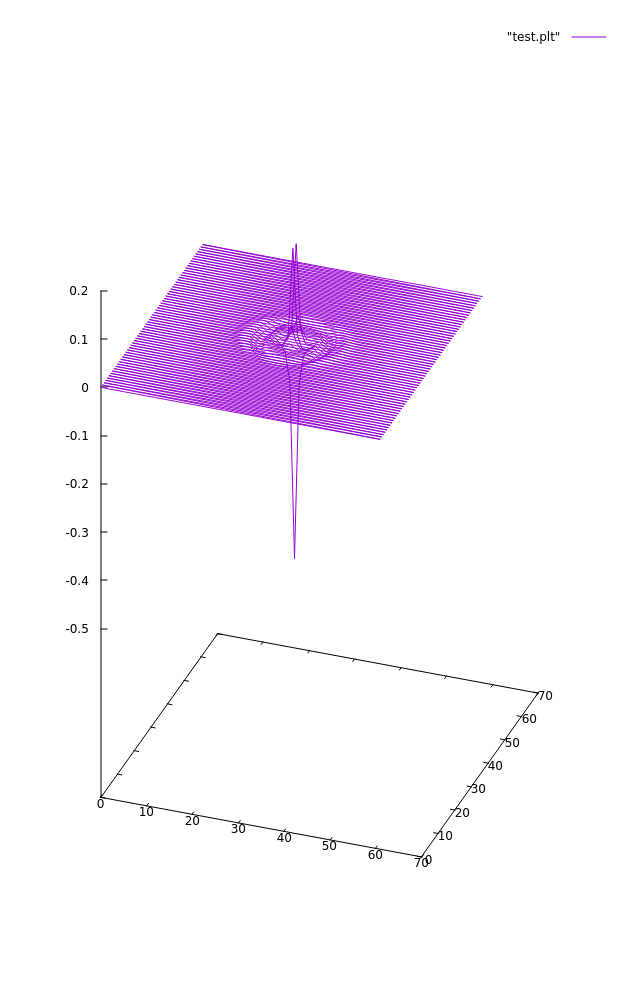
\includegraphics[width=\textwidth]{./fdtd_3d_iter_korrekt}
	\source{./main --usize 62 --samplerate\_space 20 --samplerate\_time 10 --max\_time 200 --ramped\_sin\_length 10 --ramped\_sin\_amplitude 1 --ramped\_sin\_frequency 2400000000}
	\caption{Korrekter XY-Querschnit des \(E_z\)-Feldes eines isotropen Rundstrahlers}
\end{figure}

\begin{figure}[H]
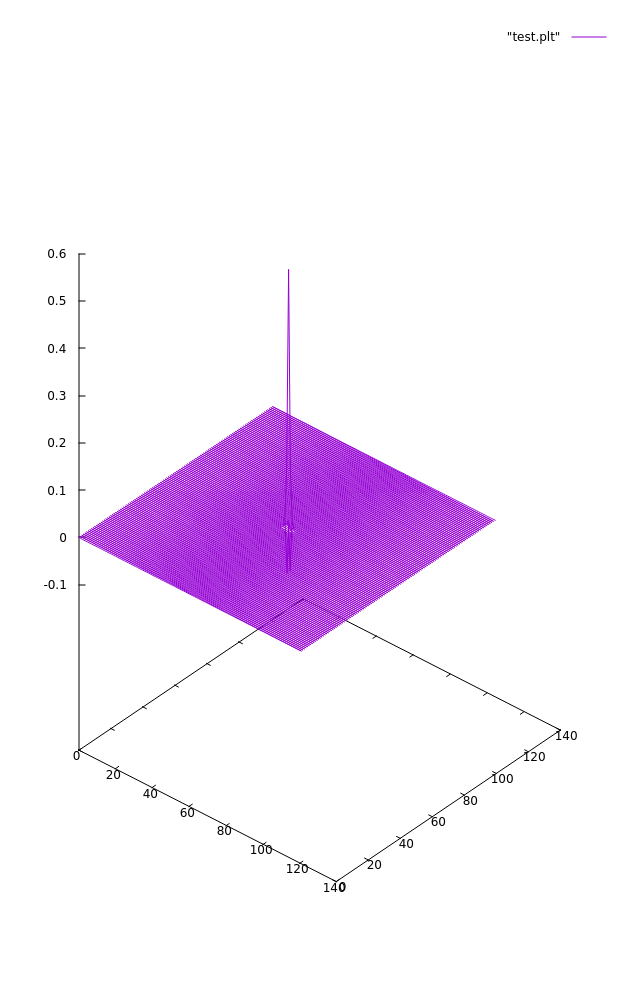
\includegraphics[width=\textwidth]{./fdtd_3d_iter_fehlerhaft}
	\source{./main --usize 122 --samplerate\_space 20 --samplerate\_time 10 --max\_time 200 --ramped\_sin\_length 10 --ramped\_sin\_amplitude 1 --ramped\_sin\_frequency 2400000000}
	\caption{Fehlerhafter XY-Querschnit des \(E_z\)-Feldes eines isotropen Rundstrahlers}
\end{figure}
\noindent Da nur der Parameter usize ver\"andert wurde, sollte sich die Form des \(E_z\)-Feldes nicht ver\"andern.

\section{Benchmarking}
Die Laufzeiten der sechs Implementierungen wurden f\"ur die selben Parameter mit dem Programm
time gemessen. Das gibt eine reale Laufzeit, sowie die Laufzeit des Prozesses im User- und im Kernelland an.
Da die Berrechnung auf die Graphikkarte ausgelagert wurden, ist nur die reale Laufzeit aussagekr\"aftig.
Alle sechs Impementierungen wurden mit den selben Parametern aufgerufen:

\begin{verbatim} 
./main --usize 62 --samplerate_space 10 --samplerate_time 20
--max_time 10000 --ramped_sin_length 100 --ramped_sin_amplitude 1
--ramped_sin_frequency 2400000000
\end{verbatim}
Das f\"uhrte zu folgenden Laufzeiten:

\begin{center}
	\begin{tabular}{c|c|c|c|}
		Flie{\ss}kommagenauigkeit & CPU & GPU ein Zeitschritt & GPU alle Zeitschritte\\
		\hline
		float & 11429100us & 11353us & 701052us\\
		double & 11348500us & 91852us & 1305535us\\
	\end{tabular}
\end{center}
Daraus l\"asst sich der Performanzgewinn errechnen

\begin{center}
	\begin{tabular}{c|c|c|c|}
		Flie{\ss}kommagenauigkeit & \(CPU/GPU_{ein}\) & \(CPU/GPU_{alle}\) & \(GPU_{ein}/GPU_{alle}\)\\
		\hline
		float & 16.302784957463924 &  1006.7030740773364 & 61.750374350391965\\
		double & 8.692604947397044 & 123.55201846448635 & 14.213462962156513\\
	\end{tabular}
\end{center}
Wird die Berrechnung aller Zeitschritte auf die GPU ausgel\"agert und Flie{\ss}kommazahlen einfacher Genauigkeit
verwendet ist die Simulation ungefaher um den Faktor 1006 beschleunigt. Sollen dagegen Flie{\ss}kommazahlen doppelter Genauigkeit
verwendet werden, so ist sie nur ungef\"ahr um den Faktor 123 beschleunigt. Flie{\ss}kommazahlen doppelter Genauigkeit sind
auf GPUs immernoch deutlich schlechter unterst\"utzt.
\newpage

\section{Simulation einer \(\lambda\)-Dipolantenne}
Eine \(\lambda\)-Dipolantenne ist ein Dipolantenne mit einer Drahtl\"ange gleich
der Wellenl\"ange der Sende- und Empfangsfrequenz.
Bei einer symmetrischen Einspeisung weist sie eine keulenf\"ormige Richtcharakteristik
auf.
Die Gittergr\"o{\ss}e wurde, wie weiter oben besprochen, so gew\"ahlt, dass die kleinste
Wellenl\"ange noch \(N_\lambda\) mal abgetastet wird. Das bedeutet um eine \(\lambda\)-Dipolantennengeometrie
zu setzen muss der Geometriefaktor von genau \(N_\lambda\) Zellen null sein. Der Simulationsbereich
ist so gro{\ss} zu w\"ahlen, dass sich das PML nicht im Nahfeld der Antenne befindet, da das die
Abstrahlcharakteristik verf\"alschen w\"urde. Der \"Ubergang von Nah- zu
Fernfeld ist dabei flie{\ss}end, f\"ur gew\"ohnlich wird angenommen, dass das Fernfeld im Radius von der dreifachen
Wellenl\"ange anf\"angt.
Die L\"ucke zwischen den beiden Armen des \(\lambda\)-Dipols
wurde nicht mitsimuliert, da sich die Antennengeometrie nicht symmetrisch teilen lie{\ss}.
Die Einspeisung des \(\lambda\)-Dipols passierte durch eine \(E_x\)-Gap Source direkt unterhalb der Mitte der
Antennengeometrie, da so die Einspeisung durch ein Koaxialkabel hinreichend gut abbildet wird.

\begin{figure}[H]
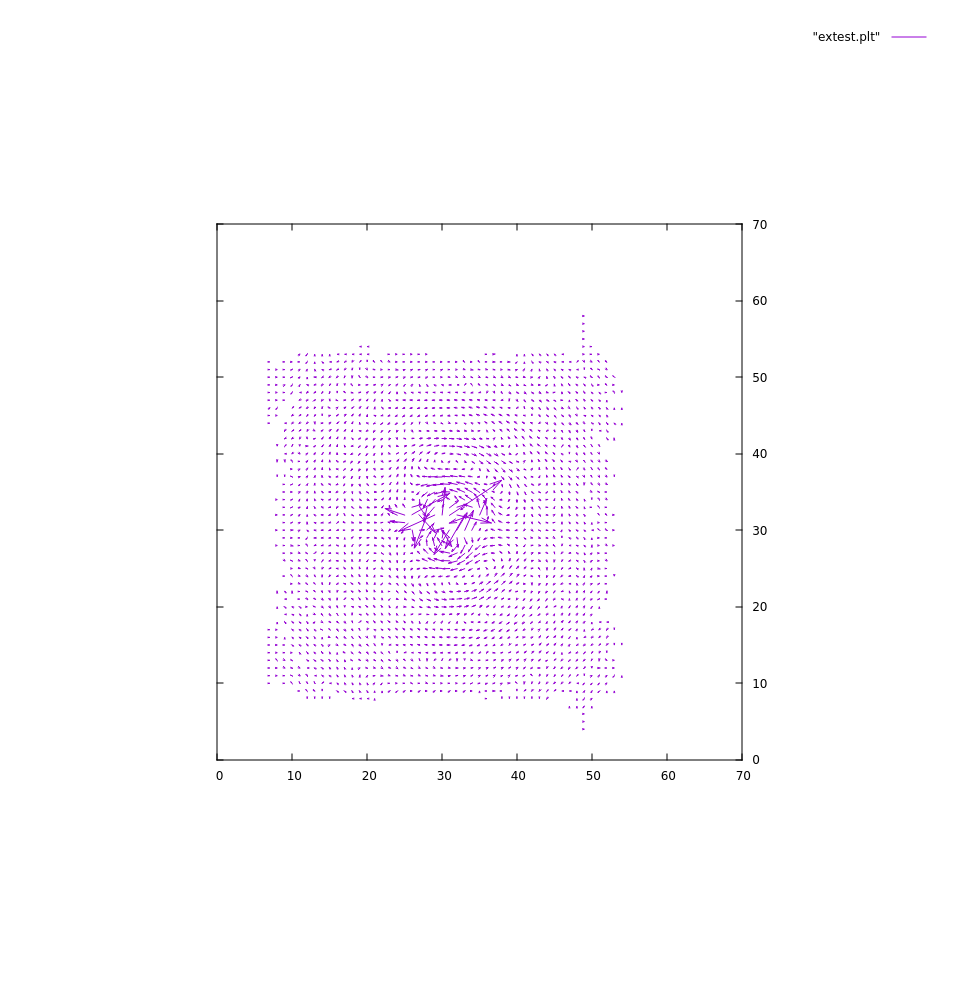
\includegraphics[width=\textwidth]{./lambda_dipol_ex_source_xyplane_efield_1.png}
	\source{\(./main --usize 62 --samplerate\_space 20 --samplerate\_time 10 --max\_time 1000 --ramped\_sin\_length 10 --ramped\_sin\_amplitude 1 --ramped\_sin\_frequency 2400000000 > extest.plt 2> ehtest.plt\)}
	\caption{Das E-Feld einer \(\lambda\)-Dipolantenne bei symmetrischer \(E\_x\)-Einspeisung}
\end{figure}
\begin{figure}[H]
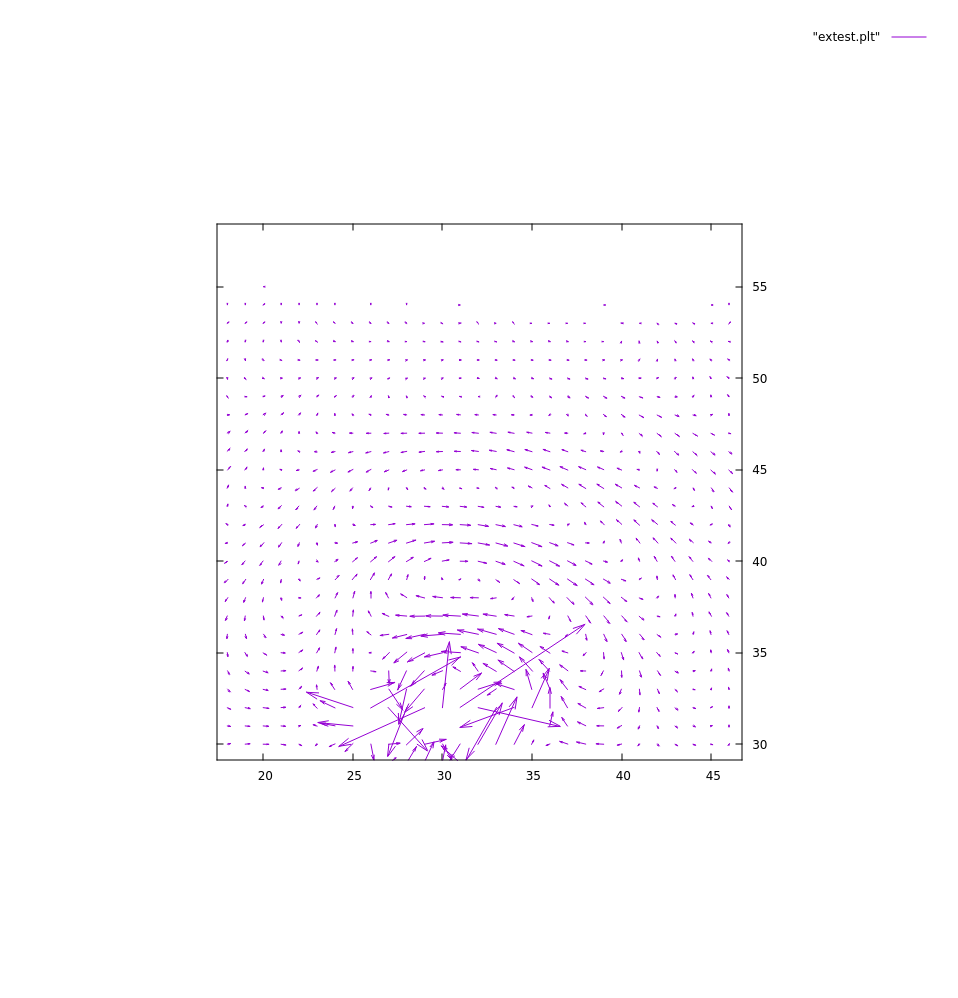
\includegraphics[width=\textwidth]{./lambda_dipol_ex_source_xyplane_efield_2.png}
	\source{\(./main --usize 62 --samplerate\_space 20 --samplerate\_time 10 --max\_time 1000 --ramped\_sin\_length 10 --ramped\_sin\_amplitude 1 --ramped\_sin\_frequency 2400000000 > extest.plt 2> ehtest.plt\)}
	\caption{Das E-Feld einer \(\lambda\)-Dipolantenne bei symmetrischer \(E\_x\)-Einspeisung (vergr\"o{\ss}er)}
\end{figure}
\noindent Das E-Feld wird in radial von der \(\lambda\)-Dipolantenne abgestrahlt. Die Richtcharakteristik l\"asst sich erahnen.

\begin{figure}[H]
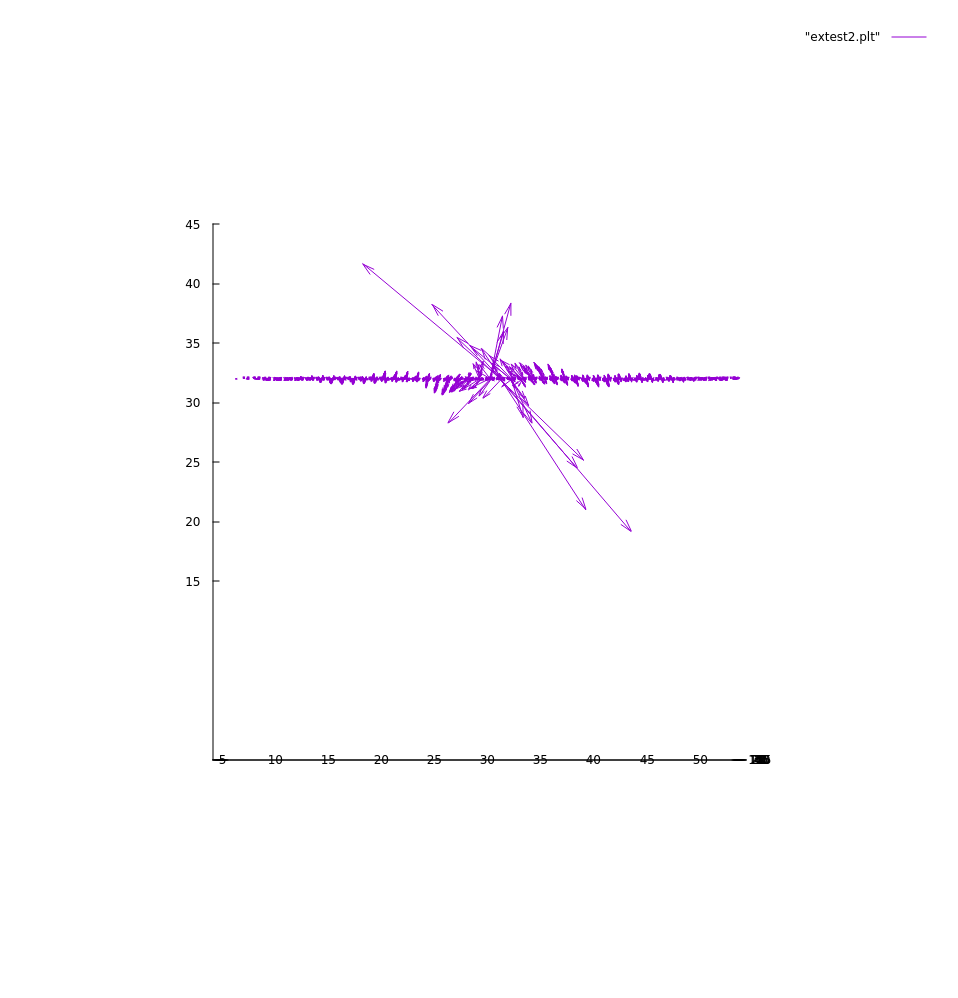
\includegraphics[width=\textwidth]{./lambda_dipol_ex_source_xyplane_hfield_1.png}
	\source{\(./main --usize 62 --samplerate\_space 20 --samplerate\_time 10 --max\_time 1000 --ramped\_sin\_length 10 --ramped\_sin\_amplitude 1 --ramped\_sin\_frequency 2400000000 > extest.plt 2> ehtest.plt\)}
	\caption{Das H-Feld einer \(\lambda\)-Dipolantenne bei symmetrischer \(E\_x\)-Einspeisung}
\end{figure}
\noindent Auch wenn man die Richtcharakteristik erahnen kann ist eine Einsch\"atzung der Abstrahlcharakteristik mit diesen Simulationsergebnissen noch nicht
m\"oglich. Daf\"ur m\"usste aus dem E- und H-Feld das Poyntingvektorfeld errechnet und in Bezug zum Feld des isotropen Rundstrahler gesetzt werden.
Auch das k\"onnte hardwarebeschleunigt implementiert werden.

\section{Zusammenfassung und Ausblicke}
Die FDTD-Methode kann theoretisch beliebig komplexe Antennegeometrien simulieren, bei gekr\"ummten Geometrien kommt es jedoch aufgrund
des Yee-Gitters zu Ungenauigkeiten. Diese k\"onnen reduziert werden, indem die r\"aumliche Abtastrate erh\"oht wird, oder aber Techniken
wie `Dielectrical Smoothing' verwendet werden.\cite{dielectrical_smoothing}. Sollen ebenfalls nichtmetallische Strukturen wie
zum Beispiel das Geh\"ause der Antenne mitsimuliert werden, so kann es ebenfalls aufgrund des Yee-Gitters zu
Ungenauigkeiten kommen. Da das E-Gitter und das H-Gitter um die H\"alfte der Gittergr\"o{\ss}e verschoben sind, kann
es sein, das Zellen gleichen Indices unterschiedliche Materialien repr\"asentieren. Dieses Problem kann durch die
`2xGrid Technique' gel\"ost werden. Dabei wird die Geometrie auf einem Yee-Gitter doppelter Aufl\"osung definiert und dann in ein
Yee-Gitter einfacher Aufl\"osung transformiert.
Nutzt man die FDTD-Methode, um unbekannte Antennen zu simulieren, hat man weiterhin das Problem, dass aus einer Simulation
nicht geschlossen werden kann, ob sich die Antenne schon eingeschwungen hat. Dieses Problem kann gel\"ost werden, indem man
die Abstrahlcharakteristik errechnet und die Simulationsdauer so lange erh\"oht, bis sich die Abstrahlcharakteristik nicht
mehr \"andert. Sollte man die FDTD-Methode als Grundlage f\"ur einen evolution\"aren Algorithmus nutzen, m\"usste dies
automatisiert passieren. Mathematisch hat sich das L\"osen der Maxwellgleichungen auf Additionen und Multiplikationen
heruntergebrochen, es w\"are daher denkbar die FDTD-Methode auf einem FPGA zu implementieren.
Jede Zelle des Yee-Gitters k\"onnte durch die Instanz einer Entity beschrieben werden, diese m\"usste nur mit den sechs benachbarten Instanzen sowie einem
Kontrolleur kommunizieren k\"onnen. Zu Beginn der Simulation w\"urde jede Instanz die PML-Vorfaktoren vom Kontrolleur erhalten,
danach k\"onnten alle Instanzen durch einen Takt synchronisiert das H-Feld und E-Feld errechnen und ihre intern gespeicherten
alten Feldst\"arken \"uberschreiben. Da moderne FPGA-Boards neben der programmierbaren Logik meist noch einen Prozessor
besitzen, k\"onnte die Interaktion mit dem Benutzer, oder aber eventuell das Zuweisen einer Fitnessfunktion auf
dem Prozessor passieren. Abschlies{\ss}end l\"asst sich sagen, die FDTD-Methode ist ein sehr m\"achtiges Verfahren und in der Lage beliebige Anntennengeometrien
zu simulieren, sie ist dabei jedoch auch so rechenintensiv, dass eine sequentielle Implementierung kaum zu verwenden ist.

%\bibliographystyle{plain}
\bibliography{cites}
\bibliographystyle{unsrtnat}
\end{document}
